\documentclass[11pt,a4paper]{article}
\usepackage{authblk}
% \usepackage[utf8]{inputenc}
\usepackage{amsthm}
\usepackage{amsfonts}
\usepackage{amsmath}
\usepackage{amssymb}
\let\amssquare\square
\usepackage{mathtools}
% \usepackage{stmaryrd}
% \usepackage{tensor}
\usepackage[mathscr]{eucal}
\usepackage{url}
% \usepackage{marvosym}
\usepackage[left=2cm,right=2cm,top=2cm,bottom=2cm]{geometry}
\usepackage{minted}

\usepackage{tikz-cd}
\usetikzlibrary{positioning}
\usetikzlibrary{fit}
\usetikzlibrary{cd}
\usetikzlibrary{arrows}
\usetikzlibrary{calc}
\usetikzlibrary{decorations.markings}
\tikzset{ed/.style={auto,inner sep=2pt,font=\scriptsize}} %edges
\tikzset{>=stealth'}
\tikzset{vert/.style={draw,circle, minimum size=6mm, inner sep=0pt, fill=white}}
\tikzset{vertbig/.style={draw,circle, minimum size=8mm, inner sep=0pt, fill=white}}
\tikzset{->-/.style={decoration={
      markings,
      mark=at position #1 with {\arrow{>}}},postaction={decorate}}}

\theoremstyle{plain}
\newtheorem{theorem}{Theorem}[subsection]
% \newtheorem{axiom}[theorem]{Axiom}
\newtheorem*{theoremstar}{Theorem}
% \newtheorem{fact}[theorem]{Fact}
\newtheorem{proposition}[theorem]{Proposition}
\newtheorem{lemma}[theorem]{Lemma}
\newtheorem{corollary}[theorem]{Corollary}

\theoremstyle{definition}
\newtheorem{definition}[theorem]{Definition}
% \newtheorem{convention}[theorem]{Convention}
% \newtheorem{construction}[theorem]{Construction}
\newtheorem{example}[theorem]{Example}
% \newtheorem{examples}[theorem]{Examples}
% \newtheorem{notation}[theorem]{Notation}
\newtheorem{remark}[theorem]{Remark}
% \newtheorem{idea}[theorem]{Idea}
% \newtheorem{question}[theorem]{Question}

\newcommand{\C}{\mathscr{C}}
\newcommand{\homC}{\underline{\C}}
\newcommand{\D}{\mathscr{D}}
\newcommand{\E}{\mathscr{E}}
\newcommand{\M}{\mathscr{M}}
\newcommand{\N}{\mathscr{N}}
\newcommand{\T}{\mathscr{T}}

\newcommand{\bN}{\mathbb{N}}
\newcommand{\bZ}{\mathbb{Z}}


\newcommand{\Pastro}{\Phi}
% \newcommand{\Pastro}{\mathrm{Pastro}}
\newcommand{\Double}{\mathcal{D}}

% Categories
\newcommand{\Set}{\mathbf{Set}}
\newcommand{\Cat}{\mathbf{Cat}}
\newcommand{\Prof}{\mathbf{Prof}}
\newcommand{\Core}{\mathbf{Core}}
\newcommand{\MonCat}{\mathbf{MonCat}}
\newcommand{\LaxMonCat}{\mathbf{LaxMonCat}}
\newcommand{\SymmMonCat}{\mathbf{SymmMonCat}}
\newcommand{\Tele}{\mathbf{Tele}}

\newcommand{\Act}{\mathbf{Act}}
\newcommand{\Optic}{\mathbf{Optic}}
\newcommand{\Lawful}{\mathbf{Lawful}}
\newcommand{\SemiOptic}{\mathbf{SemiOptic}}
\newcommand{\Lens}{\mathbf{Lens}}
\newcommand{\Prism}{\mathbf{Prism}}
\newcommand{\Setter}{\mathbf{Setter}}
\newcommand{\Hask}{\mathbf{Hask}}
\newcommand{\Endo}{\mathbf{Endo}}
\newcommand{\Strong}{\mathbf{Strong}}
\newcommand{\Tamb}{\mathbf{Tamb}}
\newcommand{\Point}{\mathbf{Point}}
\newcommand{\CoPoint}{\mathbf{CoPoint}}
\newcommand{\Traversable}{\mathbf{Traversable}}

\newcommand{\switched}{\mathbin{\tilde{\otimes}}}

\newcommand{\id}{\mathrm{id}}
\newcommand{\op}{\mathrm{op}}
\newcommand{\const}{\mathrm{const}}
\DeclareMathOperator{\ob}{ob}
\DeclareMathOperator{\copr}{copr}
\newcommand{\inl}{\mathrm{inl}}
\newcommand{\inr}{\mathrm{inr}}
\DeclareMathOperator{\im}{im}

\newcommand{\fget}{\textsc{Get}}
\newcommand{\fput}{\textsc{Put}}
\newcommand{\fmodify}{\textsc{Modify}}
\newcommand{\freview}{\textsc{Review}}
\newcommand{\fmatching}{\textsc{Matching}}
\newcommand{\funzip}{\textsc{Unzip}}

\newcommand{\inside}{\mathsf{inside}}
\newcommand{\outside}{\mathsf{outside}}
\newcommand{\once}{\mathsf{once}}
\newcommand{\twice}{\mathsf{twice}}

% Special arrows
\newcommand{\isoto}{\xrightarrow{\cong}}
\newcommand{\hto}{\ensuremath{\,\mathaccent\shortmid\rightarrow\,}}

\makeatletter
\providecommand{\leftsquigarrow}{%
  \mathrel{\mathpalette\reflect@squig\relax}%
}
\newcommand{\reflect@squig}[2]{%
  \reflectbox{$\m@th#1\rightsquigarrow$}%
}
\makeatother

% Draft helpers
\newcommand{\todo}[1]{\textcolor{red}{\small #1}}

\newif\ifhideproofs
% \hideproofstrue %uncomment to hide proofs
\ifhideproofs
\usepackage{environ}
\NewEnviron{hide}{}
\let\proof\hide
\let\endproof\endhide
\fi

\title{Categories of Optics}
\author{Mitchell Riley}
\affil{Wesleyan University \\ \texttt{mvriley@wesleyan.edu}}
\begin{document}
\maketitle

\section{Introduction}

\todo{Past work:
  \begin{itemize}
  \item The Haskell lens people: edwardk, shachaf, xplat, roconnor... (TODO: find out who these people are)
  \item The Doubles paper
  \item Bartosz's blog post which was written about the same time I started this. (Only tensor-like optics, no discussion of laws, confusion about enrichment(?))
  \item The profunctor optics paper out of Oxford. (No generality, nothing categorical, no discussion of laws)
  \item Very old Dialectica category stuff
  \end{itemize}
}

\todo{Contributions:
  \begin{itemize}
  \item A definition of optics general enough to encompass lenses, setters, traversals, and others?
  \item A universal property satisfied by the category of optics in the monoidal case
  \item A satisfying categorical description of lens laws
  \item An attempt to isolate exactly what $\Set$-like properties are being used in various places
  \item A couple of new avenues for generalising optics
  \end{itemize}
}

A lens from $S$ to $A$ is a pair of maps $\fget : S \to A$ and $\fput : S \times A \to S$ that typically obeys three laws (whose names are in diagrammatic order):
\begin{itemize}
\item ``$\fput\fget$'': $\fget \; \fput = \pi_2$ as maps $S \times A \to A$, so that any update to $A$ should be represented faithfully in $S$;
\item ``$\fget\fput$'': $\fput [\id_S, \fget] = \id_S$ as maps $S \to S$, so that if $A$ is not changed then $S$ should not change; and,
\item ``$\fput\fput$'': $\fput (\fput \times A) = \fput \, \pi_{1, 3}$ as maps $S \times A \times A \to S$, so any update to $A$ completely overwrites previous updates.
\end{itemize}

\todo{talk about ``constant complement'' idea}

\todo{
  \subsection{(Co)ends and (Co)Yoneda}
}
If $\E$ is cocomplete, there is a formula for the coend as the coequaliser in the diagram
\[
  \begin{tikzcd}
    \coprod_{M \to N} P(N, M) \ar[r,shift left=.75ex]  \ar[r,shift right=.75ex] & \coprod_{M \in \M} P(M, M) \ar[r] & \int^{M \in \M} P(M, M)
  \end{tikzcd}
\]
where $P$ is a functor $\M^\op \times \M \to \E$.

\section{Optics}
\label{sec-optics}

We begin by constructing the category of optics in a symmetric monoidal category $\C$. This category was first defined in \cite[Section 6]{Doubles} to investigate the relationship between Tambara modules and the center of a monoidal category. There it is called the \emph{double} $\Double_l \C$ of a monoidal category, and our definition is identical, other than flipping the direction of the morphisms to match the existing work on lenses, and restricting our attention to the unenriched case.

\begin{remark}
  In what follows, we use the standard cheat of omitting associativity isomorphisms.
\end{remark}

\begin{definition}
  Let $\C$ be a symmetric monoidal category, and suppose we have two pairs of objects $(S, S')$ and $(A, A')$. An \emph{optic} $p : (S, S') \hto (A, A')$ is an element of the set
  \begin{align*}
    \Optic_\C((S, S'), (A, A')) := \int^{M \in \C} \C(S, M \otimes A) \times \C(M \otimes A', S')
  \end{align*}
\end{definition}

Because this coend takes place in $\Set$, we can describe the set $\Optic_\C((S, S'), (A, A'))$ explicitly. It is the set of pairs $(l, r)$, where $l : S \to M \otimes A$ and $r : M \otimes A' \to S'$, quotiented by the relation
\begin{align*}
  ((f \otimes A) l, r) \sim (l, r (f \otimes A'))
\end{align*}
where $l : S \to M \otimes A$, $r : N \otimes A' \to S'$ and $f : M \to N$.

If $l : S \to M \otimes A$ and $r : M \otimes A' \to S'$, we write $\langle l \mid r \rangle : (S, S') \hto (A, A')$ for the image of this pair in $\Optic_\C((S, S'), (A, A'))$, and say that $M$ is the complement for the representative. Optics will always be written with a crossed arrow $\hto$, to distinguish them from morphisms of $\C$.

\begin{example}
  For any three objects $M, A, A' \in \C$, there is the \emph{tautological} optic \[t_{M,A} : (M \otimes A, M \otimes A') \hto (A, A')\] which is given by $\langle \id_{M \otimes A}\mid \id_{M \otimes A'} \rangle$.
\end{example}

\begin{remark}
  Elements of $\Optic_\C((S, S'), (A, A'))$ have an appealing
  interpretation as string diagrams with a ``hole'' missing. We draw the
  pair $\langle l \mid r \rangle$ as
  \begin{center}
    \begin{tikzpicture}
\node[vert] (l) at (0, 0) {$l$};
\node[vert] (r) at (4, 0) {$r$};

\node (S) [left of=l] {$S$};
\node (A) [below right = 0.7 and 1 of l] {$A$};
\node (S') [right of=r] {$S'$};
\node (A') [below left = 0.7 and 1 of r] {$A'$};

\draw[->] (S) -- (l);
\draw[->] (l) to[out=south east,in=west] (A);

\draw[<-] (S') -- (r);
\draw[<-] (r) to[out=south west,in=east] (A');

\draw[->] (l) to[rrel, out=north east, in=west] (1,1)
 to +(2,0)
 to[out=east, in=north west] (r)
;

\node[draw,dashed,fit=(A) (A'), inner xsep = 8pt] (box) {};
\draw[dashed] (box.90) -- +(0,2.25);
\end{tikzpicture}
  \end{center}
  reading left to right, so the left half of the diagram represents $l$ and the right half $r$. The relation imposed by the coend equates the following two diagrams:
  \begin{center}
    \begin{tikzpicture}
\begin{scope}[on grid]

\node at (0,0) (S) {$S$};
\node[rectangle,draw=black, right=of S] (l) {$l$} ;
\node[below right=of l] (A) {$A$};
\node[right= 2cm of A] (A') {$A'$};
\coordinate[above= 2cm of A] (M);
\node[rectangle,draw=black,right= 0.1cm of M] (f) {$f$};
\coordinate[above= 2cm of A'] (M');

\node[rectangle,draw=black, above right=of A']  (r) {$r$} ;
\node[right=of r] (S') {$S'$};


\draw (S) -- (l);
\draw (l.30) to [out=0,in=180] (M) -- (f.west);
\draw (f.east) -- (M') to [out=0,in=180](r.150);
\draw (l.-30) to [out=0,in=180] (A);
\draw (r.210) to [out=180,in=0] (A');
\draw (r) -- (S');

\node[draw,dashed,fit=(A) (A')] (box) {};
\draw[dashed] (box.90) -- +(0,2);

\end{scope}
\end{tikzpicture}
    \qquad
    \begin{tikzpicture}  
\begin{scope}[on grid]

\node at (0,0) (S) {$S$};
\node[rectangle,draw=black, right=of S] (l) {$l$} ;
\node[below right=of l] (A) {$A$};
\node[right= 2cm of A] (A') {$A'$};
\coordinate[above= 2cm of A] (M);
\node[rectangle,draw=black,left= 0.1cm of M'] (f) {$f$};
\coordinate[above= 2cm of A'] (M');

\node[rectangle,draw=black, above right=of A']  (r) {$r$} ;
\node[right=of r] (S') {$S'$};

\draw (S) -- (l);
\draw (l.30) to [out=0,in=180] (M) -- (f.west);
\draw (f.east) -- (M') to [out=0,in=180](r.150);
\draw (l.-30) to [out=0,in=180] (A);
\draw (r.210) to [out=180,in=0] (A');
\draw (r) -- (S');

\node[draw,dashed,fit=(A) (A')] (box) {};
\draw[dashed] (box.90) -- +(0,2);

\end{scope}
\end{tikzpicture}
  \end{center}
  We will therefore omit the vertical cut point between $l$ and $r$ in subsequent diagrams; any choice yields a representative of same optic.
\end{remark}

Two optics can be composed as follows: \todo{I give possibly too much detail here.} We wish to construct a map
\begin{align*}
  &\left(\int^{M \in \C} \C(S, M \otimes A) \times \C(M \otimes A', S')\right) \times \left(\int^{M \in \C} \C(R, M \otimes S) \times \C(M \otimes S', R')\right) \\ &
                                                                                                                                                                       \quad \to \int^{M \in \C} \C(R, M \otimes A) \times \C(M \otimes A', R').
\end{align*}
The product in $\Set$ preserves colimits, so in particular coends. Using this fact, and the Fubini theorem for coends~\cite[Remark 1.9]{CoendCofriend}, the domain is isomorphic to
\begin{align*}
  \int^{(M, N) \in \C \times \C} \C(S, M \otimes A) \times \C(M \otimes A', S') \times \C(R, N \otimes S) \times \C(N \otimes S', R').
\end{align*}
So by the universal property of coends, it suffices to construct natural maps
\begin{align*}
  & \C(S, M \otimes A) \times \C(M \otimes A', S') \times \C(R, N \otimes S) \times \C(N \otimes S', R') \\ &
                                                                                                              \quad \to \int^{M \in \C} \C(R, M \otimes A) \times \C(M \otimes A', R').
\end{align*}
for each $M, N \in \C$. For this we use the composites
\begin{align*}
  &\C(S, M \otimes A) \times \C(M \otimes A', S') \times \C(R, N \otimes S) \times \C(N \otimes S', R')\\
  \to \,& \C(N \otimes S, N \otimes M \otimes A) \times \C(N \otimes M \otimes A', N \otimes S') \times \C(R, N \otimes S) \times \C(N \otimes S', R') && \text{(functoriality of $N \otimes  -$)} \\
  \to \,& \C(R, N \otimes  M \otimes A) \times \C(N \otimes M \otimes A', R') && \text{(composition in $\C$)} \\
  \to \,&\int^{M \in \M} \C(R, M \otimes A) \times \C(M \otimes A', R') && \text{($\copr_{N \otimes M}$)}
\end{align*}
In other words, let $\langle l', r' \rangle : (R, R') \hto (S, S')$ and $\langle l, r \rangle : (S, S') \hto (A, A')$ with $M$ the complement for $\langle l', r' \rangle$. The composite is then: $\langle l, r \rangle \circ \langle l', r' \rangle = \langle (M l)l', r'(Mr)\rangle$.

Graphically, this is placing the first optic into the hole of the second:
\begin{center}
  \begin{tikzpicture}
\node[vert] (l) at (0, 0) {$l$};
\node[vert] (r) at (4, 0) {$r$};

\node (S) [left of=l] {$S$};
\node (A) [below right = 0.7 and 1 of l] {$A$};
\node (S') [right of=r] {$S'$};
\node (A') [below left = 0.7 and 1 of r] {$A'$};

\draw[->] (S) -- (l);
\draw[->] (l) to[out=south east,in=west] (A);

\draw[<-] (S') -- (r);
\draw[<-] (r) to[out=south west,in=east] (A');

\draw[->] (l) to[rrel, out=north east, in=west] (1,1)
 to +(2,0)
 to[out=east, in=north west] (r)
;

\node[draw,dashed,fit=(A) (A'), inner xsep = 8pt] (box) {};
\end{tikzpicture}
  \qquad\raisebox{1.5cm}{$\circ$}\qquad
  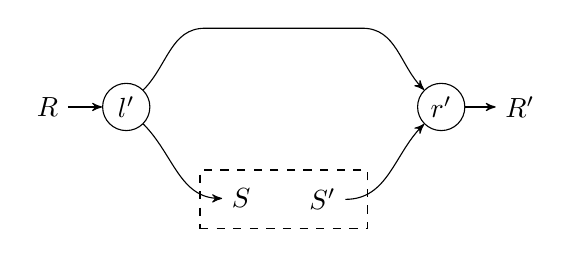
\begin{tikzpicture}
\node[vert] (l) at (0, 0) {$l'$};
\node[vert] (r) at (4, 0) {$r'$};

\node (R) [left of=l] {$R$};
\node (S) [below right = 0.7 and 1 of l] {$S$};
\node (R') [right of=r] {$R'$};
\node (S') [below left = 0.7 and 1 of r] {$S'$};

\draw[->] (R) -- (l);
\draw[->] (l) to[out=south east,in=west] (S);

\draw[<-] (R') -- (r);
\draw[<-] (r) to[out=south west,in=east] (S');

\draw[->] (l) to[out=north east, in=west] ++(1,1)
 to ++(2,0)
 to[out=east, in=north west] (r)
;

\node[draw,dashed,fit=(S) (S'), inner xsep = 8pt] (box) {};
\end{tikzpicture} \\
  \raisebox{1.5cm}{$:=$}\qquad
  \begin{tikzpicture}
\begin{scope}[on grid]

\node[vert] (l') at (0, 0) {$l'$};
\node[vert, below right = 0.7 and 1 of l'] (l) {$l$};
\node[vert] (r') at (5, 0) {$r'$};
\node[vert, below left = 0.7 and 1 of r'] (r) {$r$};

\node (A) [below right = 0.7 and 1 of l] {$A$};
\node (A') [below left = 0.7 and 1 of r] {$A'$};

\node (R) [left of=l'] {$R$};
\node (R') [right of=r'] {$R'$};

\draw[->] (R) -- (l');
\draw[<-] (R') -- (r');

\draw[->] (l') to[rrel, out=north east, in=west] (1,1)
 to +(3,0)
 to[out=east, in=north west] (r')
;

\draw[->] (l) to[rrel, out=north east, in=west] (1,1)
 to +(1,0)
 to[out=east, in=north west] (r)
;

\draw[->] (l') to[out=south east,in=west] (l);
\draw[->] (r) to[out=east, in=south west] (r');

\draw[->] (l) to[out=south east,in=west] (A);
\draw[<-] (r) to[out=south west,in=east] (A');

\node[draw,dashed,fit=(l) (r), inner xsep = 6pt, inner ysep = 25pt] (box2) {};
\node[draw,dashed,fit=(A) (A'), inner xsep = 8pt] (box) {};
\end{scope}
\end{tikzpicture}
\end{center}

The identity optic $(S, S') \hto (S, S')$ is given by $\langle \lambda^{-1}_S, \lambda_{S'} \rangle$, where $\lambda_S : I \otimes S \to S$ is the left unitor for $S$:
\begin{center}
  \begin{tikzpicture}
\begin{scope}[on grid]
\node[vert] (l) at (0, 0) {$\lambda_S^{-1}$};
\node[vert] (r) at (4, 0) {$\lambda_{S'}$};

\node (S) [left of=l] {$S$};
\node (A) [below right = 0.7 and 1 of l] {$S$};
\node (S') [right of=r] {$S'$};
\node (A') [below left = 0.7 and 1 of r] {$S'$};

\draw[->] (S) -- (l);
\draw[->] (l) to[out=south east,in=west] (A);

\draw[<-] (S') -- (r);
\draw[<-] (r) to[out=south west,in=east] (A');

\draw[->, dotted] (l) to[rrel, out=north east, in=west] (1,1)
 to +(2,0)
 to[out=east, in=north west] (r)
;

\node[draw,dashed,fit=(A) (A'), inner xsep = 8pt] (box) {};
\end{scope}
\end{tikzpicture}
\end{center}
This dashed line above the diagram represents the unit object. As is standard, we will elide the unit object and unitors in future diagrams unless they are necessary. The diagram for the identity becomes:
\begin{center}
  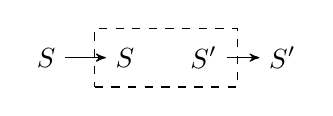
\begin{tikzpicture}
\node (Sin) {$S$};
\node (Sout) [right of=Sin] {$S$};
\node (Spout) [right of=Sout] {$S'$};
\node (Spin) [right of=Spout] {$S'$};

\draw[->] (Sin) -- (Sout);
\draw[->] (Spout) -- (Spin);

\node[draw,dashed,fit=(Sout) (Spout), inner xsep = 4pt] (box) {};
\end{tikzpicture}
\end{center}

\begin{proposition}
  The above data form a category $\Optic_\C$.
\end{proposition}
\begin{proof}
  In~\cite[Section 6]{Doubles} this is proven abstractly, by exhibiting this category as the Kleisli category for a monad in the bicategory $\Prof$. Here we prove the properties directly.

  We check associativity of composition equationally. As in the definition of composition, the Fubini theorem for coends allows us to choose representatives for all three optics simultaneously. Suppose we have representatives of three optics $\langle l_1, r_1\rangle : (R, R) \hto (S, S')$ and $\langle l_2, r_2 \rangle : (S, S') \hto (A, A')$ and $\langle l_3, r_3 \rangle : (A, A') \hto (B, B')$, that have complements $M$, $N$ and $P$ respectively. Then:
  \begin{align*}
    (\langle l_3, r_3 \rangle \circ \langle l_2, r_2 \rangle) \circ \langle l_1, r_1 \rangle
    &= \langle (N \otimes l_3)l_2, r_2(N \otimes r_3) \rangle \circ \langle l_1, r_1 \rangle \\
    &= \langle (M \otimes ((N \otimes l_3)l_2))l_1, r_1(M \otimes (r_2(N \otimes r_3))) \rangle \\
    &= \langle (M \otimes N \otimes l_3)(M \otimes l_2)l_1, r_1(M \otimes r_2)(M \otimes N \otimes r_3) \rangle \\
    &= \langle l_3, r_3 \rangle \circ (\langle (M \otimes l_2)l_1, r_1(M \otimes r_2) \rangle) \\
    &= \langle l_3, r_3 \rangle \circ (\langle l_2, r_2 \rangle \circ \langle l_1, r_1 \rangle)
  \end{align*}

  For the unit laws, suppose we have $\langle l, r \rangle : (S, S') \hto (A, A')$ with representative $M$. We calculate:
  \begin{align*}
    \id_{A, A'} \circ \langle l, r\rangle
    &= \langle \lambda^{-1}_A, \lambda_{A'} \rangle \circ \langle l, r\rangle \\
    &= \langle (M \otimes \lambda^{-1}_A) l, r (M\otimes  \lambda_{A'})\rangle \\
    &= \langle (\lambda^{-1}_M \otimes  A) l, r (\lambda_M \otimes A')\rangle \\
    &= \langle l, r (\lambda_M \otimes A') (\lambda^{-1}_M \otimes A')\rangle \\
    &= \langle l, r \rangle  \\
    \langle l, r \rangle \circ \id_{S, S'}
    &= \langle l, r \rangle \circ \langle \lambda^{-1}_S, \lambda_{S'}\rangle  \\
    &= \langle (I \otimes l)\lambda^{-1}_S, \lambda_{S'} (I \otimes r) \rangle \\
    &= \langle (\lambda^{-1}_M \otimes S)l, r (\lambda_{M} \otimes S') \rangle \\
    &= \langle l, r (\lambda_{M} \otimes S')(\lambda^{-1}_M \otimes S') \rangle \\
    &= \langle l, r \rangle
  \end{align*}
  Where in both cases we have used the naturality of $\lambda$ and coend relations to move $\lambda^{-1}_M$ to the right-hand side of the coend, where it may be cancelled.
\end{proof}

\begin{remark}
  Note that the homsets of $\Optic_\C$ are given by a coend indexed by a possibly large category, so their existence is not guaranteed by the cocompleteness of $\Set$. We should be careful to only discuss $\Optic$ categories where we know that the coends exist by some other means, e.g., by exhibiting an isomorphism with some other set. For many---but not all---of the examples given later, we provide such an isomorphism.

  \todo{How does the doubles paper get away with it?}
\end{remark}

The remainder of this section comprises some useful observations that were not made in~\cite{Doubles}.

\begin{proposition}
  There is a functor $\iota : \C \times \C^\op \to \Optic_\C$, which is given on objects by $\iota(S, S') = (S, S')$ and for a morphism $(f, g) : (S, S') \to (A, A')$ by $\iota(f, g) = \langle \lambda_A^{-1} f, g \lambda_{A'} \rangle$.
\end{proposition}
\begin{proof}
  Graphically, this is:
  \begin{center}
    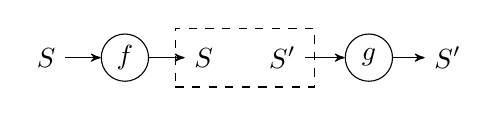
\begin{tikzpicture}
\node (Sin) {$S$};
\node (f) [vert, right of=Sin] {$f$};
\node (Sout) [right of=f] {$S$};
\node (Spout) [right of=Sout] {$S'$};
\node (g) [vert, right = 0.5 of Spout] {$g$};
\node (Spin) [right of=g] {$S'$};

\draw[->] (Sin) -- (f);
\draw[->] (f) -- (Sout);
\draw[->] (Spout) -- (g);
\draw[->] (g) -- (Spin);

\node[draw,dashed,fit=(Sout) (Spout)] (box) {};
\end{tikzpicture}
  \end{center}

  This preserves identities, as the identity on an object $(S, S')$ in $\Optic_\M$ is defined to be exactly $\langle \lambda^{-1}_S, \lambda_{S'} \rangle$. To check functoriality, suppose we have $(f, g) : (S, S') \to (A, A')$ and $(f', g') : (A, A') \to (B, B')$ in $\C \times \C^\op$. Then:
  \begin{align*}
    \iota(f', g') \circ \iota(f, g)
    &= \langle \lambda^{-1}_B f', g' \lambda_{B'} \rangle \circ \langle \lambda^{-1}_A f, g \lambda_{A'} \rangle \\
    &= \langle (I\otimes (\lambda^{-1}_B f'))\lambda^{-1}_A f, g \lambda_{A'} (I\otimes (g' \lambda_{B'}))\rangle && \text{(By definition of $\circ$)}\\
    &= \langle (I \otimes \lambda^{-1}_B) (I \otimes f')\lambda^{-1}_A f, g \lambda_{A'} (I \otimes g')(I\otimes \lambda_{B'})\rangle && \text{(Functoriality of $I \otimes -$)}\\
    &= \langle (I\otimes \lambda^{-1}_B) \lambda^{-1}_B f' f, g g' \lambda_{B'} (I\otimes \lambda_{B'})\rangle && \text{(Naturality of $\lambda$)}\\
    &= \langle (\lambda^{-1}_I \otimes B) \lambda^{-1}_B f' f, g g' \lambda_{B'} (\lambda_I \otimes B')\rangle && \text{(Unitality of action)} \\
    &= \langle \lambda^{-1}_B f' f, g g' \lambda_{B'} (\lambda_I \otimes B') (\lambda^{-1}_I \otimes B') \rangle && \text{(Coend relation)}  \\
    &= \langle \lambda^{-1}_B f'f, g g' \lambda_{B'} \rangle \\
    &= \iota(f'f, gg')
  \end{align*}
  Graphically, there is not much to do:
  \begin{center}
    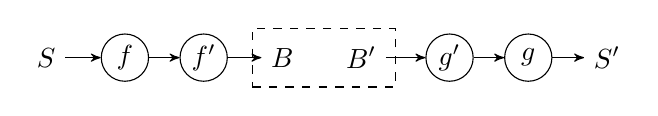
\begin{tikzpicture}
\node (Sin) {$S$};
\node (f) [vert, right of=Sin] {$f$};
\node (f') [vert, right of=f] {$f'$};
\node (Sout) [right of=f'] {$B$};
\node (Spout) [right of=Sout] {$B'$};
\node (g') [vert, right = 0.5 of Spout] {$g'$};
\node (g) [vert, right of=g'] {$g$};
\node (Spin) [right of=g] {$S'$};

\draw[->] (Sin) -- (f);
\draw[->] (f) -- (f');
\draw[->] (f') -- (Sout);
\draw[->] (Spout) -- (g');
\draw[->] (g') -- (g);
\draw[->] (g) -- (Spin);

\node[draw,dashed,fit=(Sout) (Spout)] (box) {};
\end{tikzpicture}
    \qquad \raisebox{0.3cm}{$=$} \qquad
    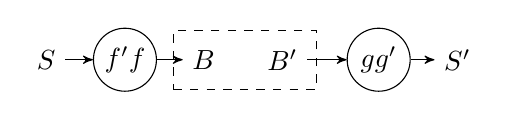
\begin{tikzpicture}
\node (Sin) {$S$};
\node (f) [vertbig, right of=Sin] {$f'f$};
\node (Sout) [right of=f] {$B$};
\node (Spout) [right of=Sout] {$B'$};
\node (g) [vertbig, right = 0.5 of Spout] {$gg'$};
\node (Spin) [right of=g] {$S'$};

\draw[->] (Sin) -- (f);
\draw[->] (f) -- (Sout);
\draw[->] (Spout) -- (g);
\draw[->] (g) -- (Spin);

\node[draw,dashed,fit=(Sout) (Spout)] (box) {};
\end{tikzpicture}
  \end{center}

\end{proof}

\begin{remark}
  This functor is not necessarily faithful, see Remark~\ref{lens-iota-not-faithful}.
\end{remark}

% \todo{This doesn't give us the structure of a `framing', we can only lift vertical arrows to horizontal arrows facing one direction.}

% \begin{theorem}
%   $\Optic_\C$ is symmetric monoidal, where $(S, S') \otimes (T, T') = (S \otimes T, S' \otimes T')$, the unit is $(I, I)$, and the action on morphisms induced by
%   \begin{align*}
%     &\C(S, M \otimes A) \times \C(M \otimes A', S') \times \C(T, N \otimes B) \times \C(N \otimes B', T')\\
%     \to \quad&\C(S \otimes T, M \otimes A \otimes N \otimes B) \times \C(M \otimes A' \otimes N \otimes B', S' \otimes T') && \text{(action of $\otimes$ on morphisms in $\C$)}\\
%     \to \quad&\C(S \otimes T, M \otimes N \otimes A \otimes B) \times \C(M \otimes N \otimes A' \otimes B', S' \otimes T') && \text{($\otimes$ in $\C$ is symmetric)}\\
%     \to \quad&\int^{M \in \C} \C(S \otimes T, M \otimes A \otimes B) \times \C(M \otimes A' \otimes B', S' \otimes T') && \text{(inclusion into coend)}
%   \end{align*}
% \end{theorem}
% \begin{proof}
%   Equationally, suppose we have representatives $(l, r) : (S \to M \otimes A, M \otimes A' \to S')$ and $(l', r') : (T \to N \otimes B, N \otimes B' \to T')$. Then:
%   \begin{align*}
%     \langle l, r \rangle \otimes \langle l', r' \rangle &:= \langle (M \otimes s_{A,N} \otimes B)(l \otimes l'), (r \otimes r')(M \otimes s_{A',N} \otimes B') \rangle
%   \end{align*}
%   This is functorial, as suggested by the equivalence of the following string diagrams:
%   \todo{todo}
%%   For future convenience, note that
%%   \begin{align*}
%%     \langle l, r \rangle \otimes (T, T') &= \langle (M \otimes s_{A,I} \otimes T)(l \otimes \lambda_T), (r \otimes \lambda^{-1}_{T'})(M \otimes s_{A',I}\otimes T') \rangle \\
%%     &= \langle (\lambda^{-1}_M \otimes A \otimes T)(M \otimes s_{A,I} \otimes T)(l \otimes \lambda_T), (r \otimes \lambda^{-1}_{T'})(M \otimes s_{A',I}\otimes T')(\lambda_M \otimes A' \otimes T') \rangle \\
%%     &= \langle l \otimes T, r \otimes T' \rangle
%%   \end{align*}
%%   Now we check functoriality. Suppose we have:
%%   \begin{align*}
%%     \langle l_1, r_1 \rangle : (S_1, S_1') &\hto (S_2, S_2') \\
%%     \langle l_2, r_2 \rangle : (S_2, S_2') &\hto (S_3, S_3') \\
%%     \langle p_1, q_1 \rangle : (T_1, T_1') &\hto (T_2, T_2') \\
%%     \langle p_2, q_2 \rangle : (T_2, T_2') &\hto (T_3, T_3')
%%   \end{align*}
%%   with complements $M_1, M_2, N_1, N_2$ respectively. Then: \todo {(This is a mess. String diagram?)}
%%   \begin{align*}
%%     &(\langle l_2, r_2 \rangle \otimes \langle p_2, q_2 \rangle) \circ (\langle l_1, r_1 \rangle \otimes \langle p_1, q_1 \rangle) \\
%%     = \; &\langle (M_2 \otimes s_{S_3,N_2} \otimes T_3)(l_2 \otimes p_2), (r_2 \otimes q_2)(M_2 \otimes s_{S_3',N_2} \otimes T_3') \rangle \\
%%     &\circ \langle (M_1 \otimes s_{S_2,N_1} \otimes T_2)(l_1 \otimes p_1), (r_1 \otimes q_1)(M_1 \otimes s_{S_2',N_1} \otimes T_2') \rangle \\
%%     = \; & \langle (M_1 \otimes N_1 \otimes M_2 \otimes s_{S_3,N_2} \otimes T_3)(M_1 \otimes N_1 \otimes l_2 \otimes p_2)(M_1 \otimes s_{S_2,N_1} \otimes T_2)(l_1 \otimes p_1), \\
%%     &\;(r_1 \otimes q_1)(M_1 \otimes s_{S_2',N_1} \otimes T_2')(M_1 \otimes N_1 \otimes r_2 \otimes q_2)(M_1 \otimes N_1 \otimes M_2 \otimes s_{S_3',N_2} \otimes T_3') \rangle \\
%%     = \; & \langle (M_1 \otimes N_1 \otimes M_2 \otimes s_{S_3,N_2} \otimes T_3)(M_1 \otimes s_{(M_2 \otimes S_3),N_1} \otimes T_3)(M_1 \otimes  l_2 \otimes N_1 \otimes p_2)(l_1 \otimes p_1), \\
%%     &\;(r_1 \otimes q_1)(M_1 \otimes r_2 \otimes N_1 \otimes q_2)(M_1 \otimes s_{(M_2 \otimes S_3'),N_1} \otimes T_3')(M_1 \otimes N_1 \otimes M_2 \otimes s_{S_3',N_2} \otimes T_3') \rangle \\
%%     = \; & \langle (M_1 \otimes N_1 \otimes M_2 \otimes s_{S_3,N_2} \otimes T_3)(M_1 \otimes s_{(M_2 \otimes S_3),N_1} \otimes T_3)((M_1 \otimes l_2)l_1\otimes (N_1 \otimes p_2)p_1), \\
%%     &\;(r_1(M_1 \otimes r_2) \otimes q_1(N_1 \otimes q_2))(M_1 \otimes s_{(M_2 \otimes S_3'),N_1} \otimes T_3')(M_1 \otimes N_1 \otimes M_2 \otimes s_{S_3',N_2} \otimes T_3') \rangle \\
%%     = \; & \text{\todo{(Add a $s_{M_2, N_1}$ to either side of the coend, then appeal to coherence)}} \\
%%     = \; &\langle (M_1 \otimes M_2 \otimes s_{(N_1 \otimes N_2),S_3} \otimes T_3)((M_1 \otimes l_2)l_1\otimes (N_1 \otimes p_2)p_1) ,  \\
%%     &\;(r_1(M_1 \otimes r_2) \otimes q_1(N_1 \otimes q_2))(M_1 \otimes M_2 \otimes s_{(N_1 \otimes N_2),S'_3} \otimes T'_3) \rangle \\
%%     = \; &\langle (M_1 \otimes l_2)l_1, r_1(M_1 \otimes r_2) \rangle \otimes \langle (N_1 \otimes p_2)p_1, q_1(N_1 \otimes q_2) \rangle \\
%%     = \; &(\langle l_2, r_2 \rangle  \circ \langle l_1, r_1 \rangle) \otimes (\langle p_2, q_2 \rangle \circ \langle p_1, q_1 \rangle)
%%   \end{align*}
%
%   The structure morphisms are all lifted from the structure morphisms in $\C$:
%   \begin{align*}
%     \alpha_{(R, R'), (S, S'), (T, T')} &:= \iota(\alpha_{R,S,T}, \alpha_{R',S',T'}^{-1}) \\
%     \lambda_{(S, S')} &:= \iota(\lambda_{(S, S')}, \lambda_{(S, S')}^{-1}) \\
%     \rho_{(S, S')} &:= (\rho_{(S, S')}, \rho_{(S, S')}^{-1}) \\
%     s_{(S, S'), (T, T')} &:= \iota(s_{S, T}, s_{T', S'})
%   \end{align*}
%
%   Note that because $\iota(S, S') = (S, S')$, required equations for $\iota$ to be a monoidal functor hold by definition (although we don't yet know that $\Optic_\otimes$ is monoidal). The pentagon and triangle axioms then hold in $\Optic_\otimes$, as they are the image of the same axioms in $\C \times \C^\op$ under $\iota$. The only remaining thing to verify is that these structure maps are natural in $\Optic_\otimes$.
%
%   Let us check that $\alpha_{(R, R'), (S, S'), (T, T')}$ is natural in $(R, R')$. Suppose $f : (Q, Q') \hto (R, R')$ has representative $(l, r) : (Q \to M \otimes R, M \otimes R' \to Q')$, then:
%   \begin{align*}
%     &\alpha_{(R, R'), (S, S'), (T, T')} \circ (f \otimes (S, S')) \otimes (T, T') \\
%     &= \iota(\alpha_{R,S,T}, \alpha_{R',S',T'}^{-1})  \circ (\langle l, r \rangle \otimes (S, S')) \otimes (T, T') \\
%     &= \langle\lambda_{R \otimes (S \otimes T)}\alpha_{R,S,T}, \alpha_{R',S',T'}^{-1} \lambda^{-1}_{(R' \otimes S') \otimes T'} \rangle  \circ \left\langle (l \otimes S) \otimes T, (r \otimes S') \otimes T' \right\rangle \\
%     &=\left\langle (M \otimes \lambda_{R \otimes (S \otimes T)}\alpha_{R,S,T})((l \otimes S) \otimes T), ((r \otimes S') \otimes T') (M \otimes \alpha_{R',S',T'}^{-1} \lambda^{-1}_{(R' \otimes S') \otimes T'} ) \right\rangle \\
%     &=\left\langle (M \otimes \alpha_{R,S,T})((l \otimes S) \otimes T), ((r \otimes S') \otimes T') (M \otimes \alpha_{R',S',T'}^{-1} )\right\rangle \\
%     &=\left\langle (l \otimes (S \otimes T))\alpha_{Q,S,T}, \alpha_{Q',S',T'}^{-1}(r \otimes (S' \otimes T')) \right\rangle \\
%     &= \langle (I \otimes l \otimes (S \otimes T)) \lambda_{Q \otimes (S \otimes T)}\alpha_{Q,S,T}, (I \times r \otimes (S' \otimes T')) \alpha_{Q',S',T'}^{-1} \lambda^{-1}_{Q' \otimes (S' \otimes T')}\rangle \\
%     &= \langle l \otimes (S \otimes T), r \otimes (S' \otimes T')\rangle \circ \left\langle \lambda_{Q \otimes (S \otimes T)}\alpha_{Q,S,T}, \alpha_{Q',S',T'}^{-1} \lambda^{-1}_{Q' \otimes (S' \otimes T')} \right\rangle \\
%     &= \langle l, r \rangle \otimes ((S, S') \otimes (T, T')) \circ \iota(\alpha_{Q,S,T}, \alpha_{Q',S',T'}^{-1}) \\
%     &= f \otimes ((S, S') \otimes (T, T')) \circ \alpha_{(Q, Q'), (S, S'), (T, T')}
%   \end{align*}
%   \todo{There is some cheating going on here, composition actually adds an extra $\alpha$, but that wouldn't get in the way.}
% \end{proof}

\begin{theorem}
  $\Optic_\C$ is symmetric monoidal, where $(S, S') \otimes (T, T') = (S \otimes T, S' \otimes T')$, the unit object is $(I, I)$, and the action on a pair of morphisms $\langle l, r \rangle : S \hto A$ and $\langle l', r' \rangle : T \hto B$ is given by:
  \begin{center}
    \begin{tikzpicture}
\begin{scope}[on grid]

\node[vert] (l) at (0, 0) {$l$};
\node[vert] (r) at (6, 0) {$r$};

\node (S) [left of=l] {$S$};
\node (A) [below right = 2 and 2 of l] {$A$};
\node (S') [right of=r] {$S'$};
\node (A') [below left = 2 and 2 of r] {$A'$};

\draw[->] (S) -- (l);
\draw[->] (l) to[out=south east,in=west] (A);

\draw[<-] (S') -- (r);
\draw[<-] (r) to[out=south west,in=east] (A');

\draw[->] (l) to[rrel, out=north east, in=west] (1,1)
 to ++(4,0)
 to[out=east, in=north west] (r)
;

\node[vert] (l') at (0, -2) {$l'$};
\node[vert] (r') at (6, -2) {$r'$};

\node (T) [left of=l'] {$T$};
\node (B) [below right = 1 and 2 of l'] {$B$};
\node (T') [right of=r'] {$T'$};
\node (B') [below left = 1 and 2 of r'] {$B'$};

\draw[->] (T) -- (l');
\draw[->] (l') to[out=south east,in=west] (B);

\draw[<-] (T') -- (r');
\draw[<-] (r') to[out=south west,in=east] (B');

\draw[->] (l') 
 to[rrel, out=north east, in=west] (2,2)
 to ++(2,0)
 to[out=east, in=north west] (r')
;

\node[draw,dashed,fit=(A) (A') (B) (B'), inner xsep = 8pt] (box) {};

\end{scope}
\end{tikzpicture}
  \end{center}
\end{theorem}
\begin{proof}
  Equationally, suppose the two optics have complements $M$ and $N$ respectively. Then:
  \begin{align*}
    \langle l, r \rangle \otimes \langle l', r' \rangle &:= \langle (M \otimes s_{A,N} \otimes B)(l \otimes l'), (r \otimes r')(M \otimes s_{A',N} \otimes B') \rangle
  \end{align*}
  This is well-defined, as the calculus of string diagrams allows us to combine the coend relation on each optic to establish the coend relation for the compound diagram. \todo{draw this?}

  Let us check functoriality of $\otimes$. Suppose we have optics:
  \begin{align*}
    \langle l_1, r_1 \rangle : (S_1, S_1') &\hto (S_2, S_2') \\
    \langle l_2, r_2 \rangle : (S_2, S_2') &\hto (S_3, S_3') \\
    \langle p_1, q_1 \rangle : (T_1, T_1') &\hto (T_2, T_2') \\
    \langle p_2, q_2 \rangle : (T_2, T_2') &\hto (T_3, T_3')
  \end{align*}
  The string diagram for $(\langle l_2, r_2 \rangle \circ \langle l_1, r_1 \rangle) \otimes (\langle p_2, q_2 \rangle \circ \langle p_1, q_1 \rangle)$ is:
  \begin{center}
    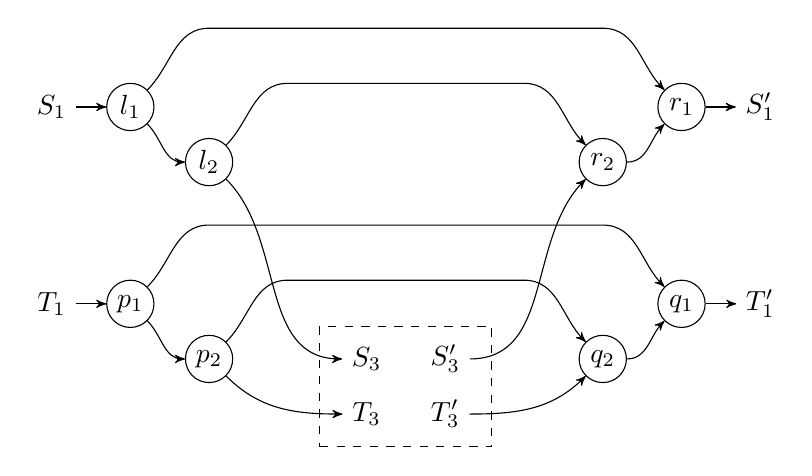
\begin{tikzpicture}
\begin{scope}[on grid]

%%% The S part

\node[vert] (l1) at (0, 0) {$l_1$};
\node[vert, below right = 0.7 and 1 of l1] (l2) {$l_2$};
\node[vert] (r1) at (7, 0) {$r_1$};
\node[vert, below left = 0.7 and 1 of r1] (r2) {$r_2$};

\node (S3) [below right = 2.5 and 2 of l2] {$S_3$};
\node (S3') [below left = 2.5 and 2 of r2] {$S_3'$};

\node (S1) [left of=l1] {$S_1$};
\node (S1') [right of=r1] {$S_1'$};

\draw[->] (S1) -- (l1);
\draw[<-] (S1') -- (r1);

\draw[->] (l1) to[out=north east, in=west] ++(1,1)
 to ($(r1) + (-1,1)$)
 to[out=east, in=north west] (r1)
;

\draw[->] (l2) to[out=north east, in=west] ++(1,1)
 to ($(r2) + (-1,1)$)
 to[out=east, in=north west] (r2)
;

\draw[->] (l1) to[out=south east,in=west] (l2);
\draw[->] (r2) to[out=east, in=south west] (r1);

\draw[->] (l2) to[out=south east,in=west] (S3);
\draw[<-] (r2) to[out=south west,in=east] (S3');

%%% The T part

\node[vert] (p1) at (0, -2.5) {$p_1$};
\node[vert, below right = 0.7 and 1 of p1] (p2) {$p_2$};
\node[vert] (q1) at (7, -2.5) {$q_1$};
\node[vert, below left = 0.7 and 1 of q1] (q2) {$q_2$};

\node (T3) [below right = 0.7 and 2 of p2] {$T_3$};
\node (T3') [below left = 0.7 and 2 of q2] {$T_3'$};

\node (T1) [left of=p1] {$T_1$};
\node (T1') [right of=q1] {$T_1'$};

\draw[->] (T1) -- (p1);
\draw[<-] (T1') -- (q1);

\draw[->] (p1) 
 to[out=north east, in=west] ++(1,1)
 to ($(q1) + (-1,1)$)
 to[out=east, in=north west] (q1)
;

\draw[->] (p2) to[out=north east, in=west] ++(1,1)
 to ($(q2) + (-1,1)$)
 to[out=east, in=north west] (q2)
;

\draw[->] (p1) to[out=south east,in=west] (p2);
\draw[->] (q2) to[out=east, in=south west] (q1);

\draw[->] (p2) to[out=south east,in=west] (T3);
\draw[<-] (q2) to[out=south west,in=east] (T3');

\node[draw,dashed,fit=(S3) (S3') (T3) (T3'), inner xsep = 8pt] (box) {};

\end{scope}
\end{tikzpicture}
  \end{center}
  And for $(\langle l_2, r_2 \rangle \otimes \langle p_2, q_2 \rangle) \circ (\langle l_1, r_1 \rangle \otimes \langle p_1, q_1 \rangle)$ is:
  \begin{center}
    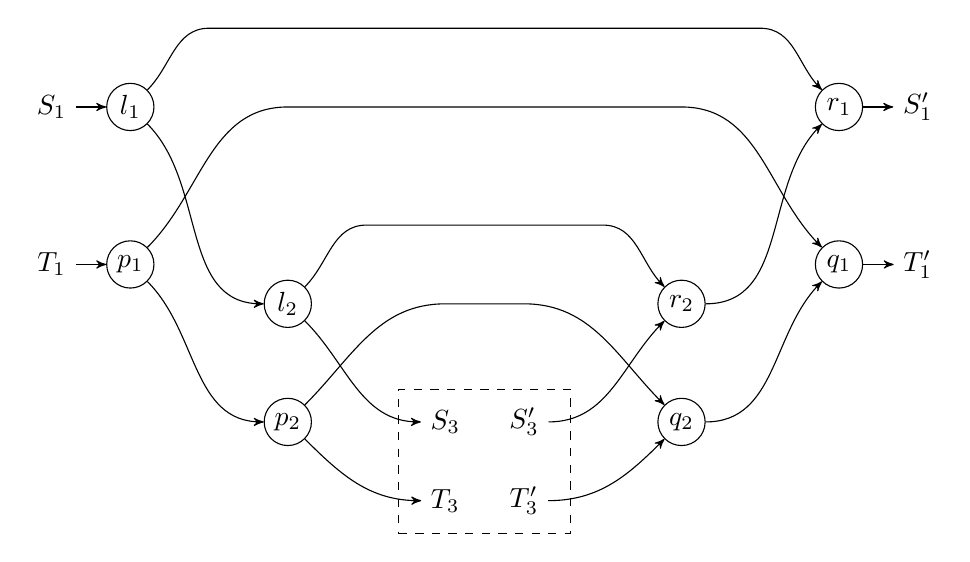
\begin{tikzpicture}
\begin{scope}[on grid]

%%% Outer:

\node[vert] (l1) at (0, 0) {$l_1$};
\node[vert] (r1) at (9, 0) {$r_1$};

\node (S1) [left of=l1] {$S_1$};
\node[vert] (l2) [below right = 2.5 and 2 of l1] {$l_2$};
\node (S1') [right of=r1] {$S_1'$};
\node[vert] (r2) [below left = 2.5 and 2 of r1] {$r_2$};

\draw[->] (S1) -- (l1);
\draw[->] (l1) to[out=south east,in=west] (l2);

\draw[<-] (S1') -- (r1);
\draw[<-] (r1) to[out=south west,in=east] (r2);

\draw[->] (l1) to[out=north east, in=west] ++(1,1)
 to ($(r1) + (-1,1)$)
 to[out=east, in=north west] (r1)
;

\node[vert] (p1) at (0, -2) {$p_1$};
\node[vert] (q1) at (9, -2) {$q_1$};

\node (T1) [left of=p1] {$T_1$};
\node[vert] (p2) [below right = 2 and 2 of p1] {$p_2$};
\node (T') [right of=q1] {$T_1'$};
\node[vert] (q2) [below left = 2 and 2 of q1] {$q_2$};

\draw[->] (T1) -- (p1);
\draw[->] (p1) to[out=south east,in=west] (p2);

\draw[<-] (T') -- (q1);
\draw[<-] (q1) to[out=south west,in=east] (q2);

\draw[->] (p1) 
 to[out=north east, in=west] ++(2,2)
 to ($(q1) + (-2,2)$)
 to[out=east, in=north west] (q1)
;

%%% Inner:

\draw[->] (l2) to[out=north east, in=west] ++(1,1)
 to ($(r2) + (-1,1)$)
 to[out=east, in=north west] (r2)
;
\draw[->] (p2) 
 to[out=north east, in=west] ++(2,1.5)
 to ($(q2) + (-2,1.5)$)
 to[out=east, in=north west] (q2)
;

\node(S3) [below right = 1.5 and 2 of l2] {$S_3$};
\node(S3') [below left = 1.5 and 2 of r2] {$S_3'$};

\draw[->] (l2) to[out=south east,in=west] (S3);
\draw[<-] (r2) to[out=south west,in=east] (S3');

\node (T3) [below right = 1 and 2 of p2] {$T_3$};
\node (T3') [below left = 1 and 2 of q2] {$T_3'$};

\draw[->] (p2) to[out=south east,in=west] (T3);
\draw[<-] (q2) to[out=south west,in=east] (T3');


\node[draw,dashed,fit=(S3) (S3') (T3) (T3'), inner xsep = 8pt] (box) {};
the a
\end{scope}
\end{tikzpicture}
  \end{center}
  These two diagrams are equivalent. We can use the naturality of the symmetry morphism to push $l_2$ and $r_2$ through to be next to $l_1$ and $r_1$ respectively. This creates two extra twists that can be cancelled in the center of the diagram.

  %%%% Note: The following is the above argument written equationally:
  % For future convenience, note that
  % \begin{align*}
  %   \langle l, r \rangle \otimes (T, T') &= \langle (M \otimes s_{A,I} \otimes T)(l \otimes \lambda_T), (r \otimes \lambda^{-1}_{T'})(M \otimes s_{A',I}\otimes T') \rangle \\
  %   &= \langle (\lambda^{-1}_M \otimes A \otimes T)(M \otimes s_{A,I} \otimes T)(l \otimes \lambda_T), (r \otimes \lambda^{-1}_{T'})(M \otimes s_{A',I}\otimes T')(\lambda_M \otimes A' \otimes T') \rangle \\
  %   &= \langle l \otimes T, r \otimes T' \rangle
  % \end{align*}
  % Now we check functoriality. Suppose we have:
  % \begin{align*}
  %   \langle l_1, r_1 \rangle : (S_1, S_1') &\hto (S_2, S_2') \\
  %   \langle l_2, r_2 \rangle : (S_2, S_2') &\hto (S_3, S_3') \\
  %   \langle p_1, q_1 \rangle : (T_1, T_1') &\hto (T_2, T_2') \\
  %   \langle p_2, q_2 \rangle : (T_2, T_2') &\hto (T_3, T_3')
  % \end{align*}
  % with complements $M_1, M_2, N_1, N_2$ respectively. Then: \todo {(This is a mess. String diagram?)}
  % \begin{align*}
  %   &(\langle l_2, r_2 \rangle \otimes \langle p_2, q_2 \rangle) \circ (\langle l_1, r_1 \rangle \otimes \langle p_1, q_1 \rangle) \\
  %   = \; &\langle (M_2 \otimes s_{S_3,N_2} \otimes T_3)(l_2 \otimes p_2), (r_2 \otimes q_2)(M_2 \otimes s_{S_3',N_2} \otimes T_3') \rangle \\
  %   &\circ \langle (M_1 \otimes s_{S_2,N_1} \otimes T_2)(l_1 \otimes p_1), (r_1 \otimes q_1)(M_1 \otimes s_{S_2',N_1} \otimes T_2') \rangle \\
  %   = \; & \langle (M_1 \otimes N_1 \otimes M_2 \otimes s_{S_3,N_2} \otimes T_3)(M_1 \otimes N_1 \otimes l_2 \otimes p_2)(M_1 \otimes s_{S_2,N_1} \otimes T_2)(l_1 \otimes p_1), \\
  %   &\;(r_1 \otimes q_1)(M_1 \otimes s_{S_2',N_1} \otimes T_2')(M_1 \otimes N_1 \otimes r_2 \otimes q_2)(M_1 \otimes N_1 \otimes M_2 \otimes s_{S_3',N_2} \otimes T_3') \rangle \\
  %   = \; & \langle (M_1 \otimes N_1 \otimes M_2 \otimes s_{S_3,N_2} \otimes T_3)(M_1 \otimes s_{(M_2 \otimes S_3),N_1} \otimes T_3)(M_1 \otimes  l_2 \otimes N_1 \otimes p_2)(l_1 \otimes p_1), \\
  %   &\;(r_1 \otimes q_1)(M_1 \otimes r_2 \otimes N_1 \otimes q_2)(M_1 \otimes s_{(M_2 \otimes S_3'),N_1} \otimes T_3')(M_1 \otimes N_1 \otimes M_2 \otimes s_{S_3',N_2} \otimes T_3') \rangle \\
  %   = \; & \langle (M_1 \otimes N_1 \otimes M_2 \otimes s_{S_3,N_2} \otimes T_3)(M_1 \otimes s_{(M_2 \otimes S_3),N_1} \otimes T_3)((M_1 \otimes l_2)l_1\otimes (N_1 \otimes p_2)p_1), \\
  %   &\;(r_1(M_1 \otimes r_2) \otimes q_1(N_1 \otimes q_2))(M_1 \otimes s_{(M_2 \otimes S_3'),N_1} \otimes T_3')(M_1 \otimes N_1 \otimes M_2 \otimes s_{S_3',N_2} \otimes T_3') \rangle \\
  %   = \; & \text{\todo{(Add a $s_{M_2, N_1}$ to either side of the coend, then appeal to coherence)}} \\
  %   = \; &\langle (M_1 \otimes M_2 \otimes s_{(N_1 \otimes N_2),S_3} \otimes T_3)((M_1 \otimes l_2)l_1\otimes (N_1 \otimes p_2)p_1) ,  \\
  %   &\;(r_1(M_1 \otimes r_2) \otimes q_1(N_1 \otimes q_2))(M_1 \otimes M_2 \otimes s_{(N_1 \otimes N_2),S'_3} \otimes T'_3) \rangle \\
  %   = \; &\langle (M_1 \otimes l_2)l_1, r_1(M_1 \otimes r_2) \rangle \otimes \langle (N_1 \otimes p_2)p_1, q_1(N_1 \otimes q_2) \rangle \\
  %   = \; &(\langle l_2, r_2 \rangle  \circ \langle l_1, r_1 \rangle) \otimes (\langle p_2, q_2 \rangle \circ \langle p_1, q_1 \rangle)
  % \end{align*}

  The structure morphisms are all lifted from the structure morphisms in $\C \times \C^\op$:
  \begin{align*}
    \alpha_{(R, R'), (S, S'), (T, T')} &:= \iota(\alpha_{R,S,T}, \alpha_{R',S',T'}^{-1}) \\
    \lambda_{(S, S')} &:= \iota(\lambda_{S}, \lambda_{S'}^{-1}) \\
    \rho_{(S, S')} &:= \iota(\rho_{S}, \rho_{S'}^{-1}) \\
    s_{(S, S'), (T, T')} &:= \iota(s_{S, T}, s_{T', S'})
  \end{align*}

  Note that because $\iota(S, S') = (S, S')$, required equations for $\iota$ to be a monoidal functor hold by definition (although we don't yet know that $\Optic_\otimes$ is monoidal). The pentagon and triangle axioms then hold in $\Optic_\otimes$, as they are the image of the same axioms in $\C \times \C^\op$ under $\iota$. The only remaining thing to verify is that these structure maps are natural in $\Optic_\otimes$.

  Let us check that $\alpha_{(R, R'), (S, S'), (T, T')}$ is natural in $(R, R')$. Suppose $f : (Q, Q') \hto (R, R')$ has representative $(l, r) : (Q \to M \otimes R, M \otimes R' \to Q')$, then:
  \begin{align*}
    &\alpha_{(R, R'), (S, S'), (T, T')} \circ (f \otimes (S, S')) \otimes (T, T') \\
    &= \iota(\alpha_{R,S,T}, \alpha_{R',S',T'}^{-1})  \circ (\langle l, r \rangle \otimes (S, S')) \otimes (T, T') \\
    &= \langle\lambda_{R \otimes (S \otimes T)}\alpha_{R,S,T}, \alpha_{R',S',T'}^{-1} \lambda^{-1}_{(R' \otimes S') \otimes T'} \rangle  \circ \left\langle (l \otimes S) \otimes T, (r \otimes S') \otimes T' \right\rangle \\
    &=\left\langle (M \otimes \lambda_{R \otimes (S \otimes T)}\alpha_{R,S,T})((l \otimes S) \otimes T), ((r \otimes S') \otimes T') (M \otimes \alpha_{R',S',T'}^{-1} \lambda^{-1}_{(R' \otimes S') \otimes T'} ) \right\rangle \\
    &=\left\langle (M \otimes \alpha_{R,S,T})((l \otimes S) \otimes T), ((r \otimes S') \otimes T') (M \otimes \alpha_{R',S',T'}^{-1} )\right\rangle \\
    &=\left\langle (l \otimes (S \otimes T))\alpha_{Q,S,T}, \alpha_{Q',S',T'}^{-1}(r \otimes (S' \otimes T')) \right\rangle \\
    &= \langle (I \otimes l \otimes (S \otimes T)) \lambda_{Q \otimes (S \otimes T)}\alpha_{Q,S,T}, (I \times r \otimes (S' \otimes T')) \alpha_{Q',S',T'}^{-1} \lambda^{-1}_{Q' \otimes (S' \otimes T')}\rangle \\
    &= \langle l \otimes (S \otimes T), r \otimes (S' \otimes T')\rangle \circ \left\langle \lambda_{Q \otimes (S \otimes T)}\alpha_{Q,S,T}, \alpha_{Q',S',T'}^{-1} \lambda^{-1}_{Q' \otimes (S' \otimes T')} \right\rangle \\
    &= \langle l, r \rangle \otimes ((S, S') \otimes (T, T')) \circ \iota(\alpha_{Q,S,T}, \alpha_{Q',S',T'}^{-1}) \\
    &= f \otimes ((S, S') \otimes (T, T')) \circ \alpha_{(Q, Q'), (S, S'), (T, T')}
  \end{align*}
  \todo{There is some cheating going on here, composition actually adds an extra $\alpha$, but that wouldn't get in the way.}

  \todo{convert this to a string diagram}
\end{proof}

\begin{remark}
  In the Haskell \texttt{lens} library, the monoidal product on optics is denoted ``\texttt{alongside}'' for the product and ``\texttt{without}'' for the coproduct.
\end{remark}

\begin{proposition}
  If $\C$ is a strict symmetric monoidal category then $\Optic_\C$ is also strict.
\end{proposition}
\begin{proof}
  The structure maps of $\Optic_\C$ are given by $\iota$ applied to the structure maps of $\C$. If the latter are identities, then so are the former---the identity morphisms in $\Optic_\C$ are by definition $\iota(\id_S, \id_S')$.
\end{proof}

\begin{proposition}
  $\iota : \C \times \C^\op \to \Optic_\C$ is a monoidal functor.
\end{proposition}
\begin{proof}
  This is clear, as the structure morphisms in $\Optic_\C$ are exactly the structure morphisms in $\C \times \C^\op$ under $\iota$.
\end{proof}

% \begin{proposition}
%   Any isomorphism $p : (S, S') \hto (A, A')$ in $\Optic_\C$ is of the form $\iota(f, g)$ for two isomorphisms $S \to A$ and $A' \to S'$ in $\C$.
% \end{proposition}
% \begin{proof}
%   \todo{This might not actually be true..}
% \end{proof}

There is some further useful structure in $\Optic_\C$.
\begin{proposition}\label{prop-costates}
  The set of costates $(S, S') \hto (I, I)$ is isomorphic to $\C(S, S')$.
\end{proposition}
\begin{proof}
  \begin{align*}
    \Optic_\C((S, S'), (I, I))
    &= \int^{M \in \C} \C(S, M \otimes I) \times \C(M \otimes I, S') \\
    &\cong \int^{M \in \C} \C(S, M) \times \C(M, S') \\
    &\cong \C(S, S')
  \end{align*}
\end{proof}

\todo{Is there a relationship between $\Optic_\C/(I, I)$ and $[2, \C]$?}

In particular, for any $S \in \C$, the image of the identity yields an optic $c_S : (S, S) \hto (I, I)$, that we will call the connector:
\begin{center}
  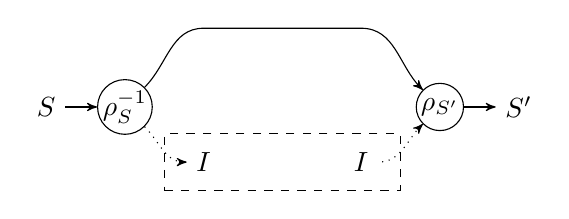
\begin{tikzpicture}
\begin{scope}[on grid]
\node[vert] (l) at (0, 0) {$\rho_S^{-1}$};
\node[vert] (r) at (4, 0) {$\rho_{S'}$};

\node (S) [left of=l] {$S$};
\node (A) [below right = 0.7 and 1 of l] {$I$};
\node (S') [right of=r] {$S'$};
\node (A') [below left = 0.7 and 1 of r] {$I$};

\draw[->] (S) -- (l);
\draw[->, dotted] (l) to[out=south east,in=west] (A);

\draw[<-] (S') -- (r);
\draw[<-, dotted] (r) to[out=south west,in=east] (A');

\draw[->] (l) to[out=north east, in=west] ++(1,1)
 to ++(2,0)
 to[out=east, in=north west] (r)
;

\node[draw,dashed,fit=(A) (A'), inner xsep = 8pt] (box) {};
\end{scope}
\end{tikzpicture}
\end{center}
Or, again omitting the unitors:
\begin{center}
  \begin{tikzpicture}
\begin{scope}[on grid]
\node (S) at (0, 0) {$S$};
\node (S') at (4, 0) {$S$};

\draw[->] (S) -- (S');

\node (I) [below right = 0.7 and 1.4 of S] {$I$};
\node (I') [below left = 0.7 and 1.4 of S'] {$I$};

\node[draw,dashed,fit=(I) (I'), inner xsep = 4pt] (box) {};
\end{scope}
\end{tikzpicture}
\end{center}

\begin{proposition}
  Suppose the monoidal unit $I$ of $\C$ is terminal. Then the set of states $(I, I) \hto (A, A')$ is isomorphic to $\C(I, A)$.
\end{proposition}
\begin{proof}
  First, note that
  \begin{align*}
    \Optic_\C((I,I), (A,A'))
    &= \int^{M \in \C} \C(I, M \otimes A) \times \C(M \otimes A', I) \\
    &\cong \int^{M \in \C} \C(I, M \otimes A).
  \end{align*}
  Because the interior of this coend is mute in the contravariant position, the coend is equal to the colimit of the functor $\C(I, - \otimes A) : \C \to \Set$. But $\C$ has a terminal object, so $\int^{M \in \C} \C(I, M \otimes A) \cong \C(I, I \otimes A) \cong \C(I, A)$.
\end{proof}

      %       \begin{proposition}
      %       \todo{Entrywise Coproduct}
      %       \end{proposition}
      %
      %       \begin{remark}
      %       The motivating example here is that of coproducts distributing over the tensor product.
      %       \end{remark}

\begin{proposition}\label{prop-change-of-action-monoidal}
  A monoidal functor $F : \C \to \D$ induces a functor $\Optic(F) : \Optic_\C \to \Optic_\D$.
\end{proposition}
\begin{proof}
  On objects this is simply $\Optic(F)(S, S') = (FS, FS')$. On a morphism $\langle l, r \rangle : (S, S') \to (A, A')$, we define
  \begin{align*}
    F\langle l, r \rangle := \langle \phi^{-1}_{M,A} (Fl), (Fr) \phi_{M,A'}\rangle
  \end{align*}
  where $\phi_{M,A} : FM \otimes FA \to F(M \otimes A)$ is the structure map of the monoidal functor.
  \todo{functoriality}
  \todo{monoidality}
\end{proof}

\begin{proposition}\label{prop-optic-functor}
  Collectively this operation defines a 2-functor \[\Optic : \SymmMonCat \to \SymmMonCat.\] \qed
\end{proposition}
\todo{Haven't actually checked natural transformations}
\todo{Also we run into the large coend issue again, it's probably not well defined on every symm mon cat.}

\subsection{Teleological Categories}
\label{teleological-categories}

In this section we establish a universal property of the $\Optic$ construction. The idea is that every optic $\langle l, r\rangle : (S, S') \hto (A, A')$ consists of a morphism $S \to M \otimes A$ and the `formal dual' of a morphism $M \otimes A' \to S'$, composed with a `formal counit' that traces out the object $M$:
\begin{center}
  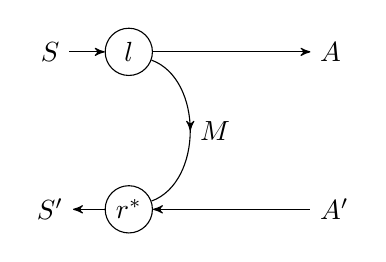
\begin{tikzpicture}
\node[vert] (l) at (0, 0) {$l$};
\node[vert] (r) at (0, -2) {$r^*$};

\node (S) [left of=l]{$S$};
\node (S') [left of=r]{$S'$};

\node (A) [right =2 of l]{$A$};
\node (A') [right = 2 of r]{$A'$};

\draw[->] (S) -- (l);
\draw[->] (l) -- (A);
\draw[<-] (S') -- (r);
\draw[<-] (r) -- (A');

\draw[->-=0.5] (l) to[out = -20, in = 20, edge label=$M$] (r);

%\node (Sin) {$S$};
%\node (f) [vert, right of=Sin] {$f$};
%\node (Sout) [right of=f] {$S$};
%\node (Spout) [right of=Sout] {$S'$};
%\node (g) [vert, right = 0.5 of Spout] {$g$};
%\node (Spin) [right of=g] {$S'$};
%
%\draw[->] (Sin) -- (f);
%\draw[->] (f) -- (Sout);
%\draw[->] (Spout) -- (g);
%\draw[->] (g) -- (Spin);
\end{tikzpicture}
\end{center}

We assume temporarily that $\C$ is a \emph{strict} symmetric monoidal category. It will be convenient to equip $\Optic_\C$ with a slightly different symmetric monoidal structure. The universal property for $\Optic_\C$ given in this section is an argument for this being the ``morally correct'' tensor, although it does seem a little strange.

\begin{definition}
  The \emph{switched} monoidal product on $\Optic_\C$ is given on objects by
  \begin{align*}
    (S, S') \switched (T, T') := (S \otimes T, T' \otimes S')
  \end{align*}
  And on morphisms $\langle l, r \rangle : S \hto A$ and $\langle l', r' \rangle : T \hto B$ by:
  \begin{center}
    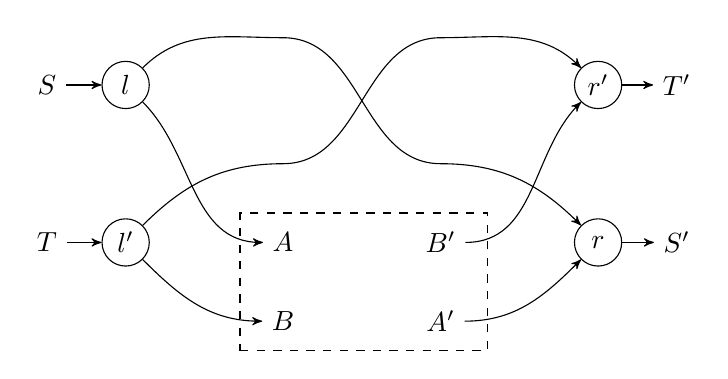
\begin{tikzpicture}
\begin{scope}[on grid]

\node[vert] (l) at (0, 0) {$l$};
\node[vert] (r') at (6, 0) {$r'$};
\node[vert] (l') at (0, -2) {$l'$};
\node[vert] (r) at (6, -2) {$r$};

\node (S) [left of=l] {$S$};
\node (A) [below right = 2 and 2 of l] {$A$};
\node (T') [right of=r'] {$T'$};
\node (B') [below left = 2 and 2 of r'] {$B'$};

\node (T) [left of=l'] {$T$};
\node (B) [below right = 1 and 2 of l'] {$B$};
\node (S') [right of=r] {$S'$};
\node (A') [below left = 1 and 2 of r] {$A'$};

\draw[->] (S) -- (l);
\draw[<-] (T') -- (r');
\draw[->] (T) -- (l');
\draw[<-] (S') -- (r);

\draw[->] (l) to[out=south east,in=west] (A);
\draw[<-] (r') to[out=south west,in=east] (B');
\draw[->] (l') to[out=south east,in=west] (B);
\draw[<-] (r) to[out=south west,in=east] (A');

\draw[->] (l') 
 to[out=north east, in=west] ++(2,1)
 to[out=east, in=west] ++(2,1.6)
 to[out=east, in=north west] (r')
;

\draw[<-] (r) 
 to[out=north west, in=east] ++(-2,1)
 to[out=west, in=east] ++(-2,1.6)
 to[out=west, in=north east] (l)
;


\node[draw,dashed,fit=(A) (A') (B) (B'), inner xsep = 8pt] (box) {};

\end{scope}
\end{tikzpicture}
  \end{center}
\end{definition}

\begin{proposition}
  $(\Optic_\C, \switched, (I, I))$ is a symmetric monoidal category that is monoidally equivalent to $\Optic_\C$ with the unswitched tensor.
\end{proposition}
\begin{proof}
  The proof that $(\Optic_\C, \switched, (I, I))$ is symmetric monoidal is nearly identical to that for the unswitched tensor. Note that due to the switching, the structure morphisms are slightly different:
  \begin{align*}
    \alpha_{(R, R'), (S, S'), (T, T')} &:= \iota(\alpha_{R,S,T}, \alpha_{T',S',R'}^{-1}) \\
    \lambda_{(S, S')} &:= \iota(\lambda_{S}, \rho_{S'}^{-1}) \\
    \rho_{(S, S')} &:= \iota(\rho_{S}, \lambda_{S'}^{-1}) \\
    s_{(S, S'), (T, T')} &:= \iota(s_{S, T}, s_{S', T'})
  \end{align*}

  The categories are monoidally equivalent via the identity functor $I : (\Optic_\C, \switched, (I, I)) \to (\Optic_\C, \otimes, (I, I))$, where the structure isomorphisms are given by
  \begin{align*}
    \iota(\id_{S \otimes S'}, s_{T, T'}) : I(S, S') \otimes I(T, T') \to I((S, S') \switched (T, T'))
  \end{align*}

\end{proof}

\begin{remark}
  Just as in the unswitched case, if $\C$ is a strict monoidal category than so is $(\Optic_\C, \switched, (I, I))$.
\end{remark}



\begin{definition}[Compare {\cite[Definition 5.1]{CoherenceForLenses}}]
  A \emph{teleological category is} a symmetric monoidal category $(\C, \otimes, I)$, equipped with:
  \begin{itemize}
  \item A wide symmetric monoidal subcategory $\C_d$ of \emph{dualisable morphisms}, with an involutive strong symmetric monoidal functor ${(-)}^* : \C_d \to \overline{\C_d^\op}$, where---not finding a standard symbol for such a thing---we mean $\overline{\C_d^\op}$ to be the category with both the direction of the arrows \emph{and} the order of the tensor flipped: ${(A \otimes B)}^* = B^* \otimes A^*$. \todo{Do we want this to be strict?}
  \item A symmetric monoidal extranatural family of morphisms $\varepsilon_X : X \otimes X^* \to I$, called \emph{counits}, natural with respect to the morphisms in $\C_d$.
  \end{itemize}
\end{definition}
Unpacking the definition, $\varepsilon$ being a symmetric monoidal extranatural transformation amounts to the following diagrams in $\C$ commuting:
\[
  \begin{tikzcd}
    X \otimes Y^* \ar[r, "f \otimes Y^*"]  \ar[d, "X \otimes f^*", swap] & Y \otimes Y^* \ar[d, "\varepsilon_Y"] \\
    X \otimes X^* \ar[r, "\varepsilon_X", swap] & I
  \end{tikzcd} \hspace{1cm}
  \begin{tikzcd}
    X^* \otimes X \ar[r, "\sigma"]  \ar[dr, "\varepsilon_{X^*}", swap] & X \otimes X^* \ar[d, "\varepsilon_X"] \\
    & I
  \end{tikzcd} \hspace{1cm}
  \begin{tikzcd}
    X \otimes Y \otimes Y^* \otimes X^* \ar[r, "X \otimes \varepsilon_Y \otimes X^*"]  \ar[dr, "\varepsilon_{X \otimes Y}", swap] & X \otimes X^* \ar[d, "\varepsilon_X"] \\
    & I
  \end{tikzcd}
\]
where $f : X \to Y$ is in $\C_d$.

%%%% The following is a version with duality given by reflection.
% \begin{definition}[{\cite[Definition 5.1]{CoherenceForLenses}}]
%   A \emph{teleological category is} a symmetric monoidal category $(\C, \otimes, I)$, equipped with:
%   \begin{itemize}
%   \item A wide symmetric monoidal subcategory $\C_d$ of \emph{dualisable morphisms}, with an involutive strong symmetric monoidal functor $(-)^* : \C_d \to \C_d^\op$; and,
%   \item A family of morphisms $\varepsilon_X : X \otimes X^* \to I$, called \emph{counits}, natural with respect to the morphisms in $\C_d$, such that
%     \[
%       \begin{tikzcd}
%         X \otimes Y^* \ar[r, "f \otimes Y^*"]  \ar[d, "X \otimes f^*", swap] & Y \otimes Y^* \ar[d, "\varepsilon_Y"] \\
%         X \otimes X^* \ar[r, "\varepsilon_X", swap] & I
%       \end{tikzcd} \hspace{1cm}
%       \begin{tikzcd}
%         X^* \otimes X \ar[r, "s_{X^*, X}"]  \ar[dr, "\varepsilon_{X^*}", swap] & X \otimes X^* \ar[d, "\varepsilon_X"] \\
%         & I
%       \end{tikzcd}
%     \]
%     \[
%       \begin{tikzcd}
%         X \otimes Y \otimes X^* \otimes Y^* \ar[r, "X \otimes s_{Y,X^*} \otimes X^*"]  \ar[dr, "\varepsilon_{X \otimes Y}", swap] & X \otimes X^* \otimes Y \otimes Y^* \ar[d, "\varepsilon_X \otimes \varepsilon_Y"] \\
%         & I
%       \end{tikzcd}
%     \]
%     commute for all $f : X \to Y$ is in $\C_d$.
%   \end{itemize}
% \end{definition}

% \begin{remark}
%   Compact closed categories very nearly form examples of teleological categories. In a compact closed category, there are canonical isomorphisms $(X \otimes Y)^* \cong Y^* \otimes X^*$. In a teleological category, however, duality does not reverse the order of the tensor. \todo{If $\C$ is strict, as it is here, does this matter?}
% \end{remark}

Note that because $\C_d$ is symmetric monoidal and has the same collection of objects as $\C$, the symmetric monoidal structure morphisms of $\C$ must all be in $\C_d$.

\begin{example}
  Any symmetric monoidal category with terminal monoidal unit is trivially teleological, setting the dualisable morphisms to be the structure maps of the monoidal category.
\end{example}

\begin{example}
  Any compact closed category is a teleological category, where every morphism is dualisable and the unit morphisms have been forgotten.
\end{example}

\todo{\begin{example}
    The funny graph example from the coherence paper?
  \end{example}}

\begin{definition}
  A \emph{teleological functor} $F : \C \to \D$ is a symmetric monoidal functor that restricts to a functor $F_d : \C_d \to \D_d$ on the dualisable subcategories, and such that $F(\varepsilon_X) = \varepsilon_{FX}$ \todo{up to the structure isomorphisms of $F$}
\end{definition}

Together we have $\Tele$, the subcategory of $\SymmMonCat$ given by teleological categories and teleological functors. There are evident functors $U : \Tele \to \SymmMonCat$ and ${(-)}_d : \Tele \to \SymmMonCat$, that take a teleological category to its underlying symmetric monoidal category and subcategory of dualisable morphisms respectively.

\begin{proposition}
  $\Optic_\C$ forms a teleological category, where:
  \begin{itemize}
  \item The dualisable morphisms are all morphisms of the form $\iota(f, g)$;
  \item The involution is given on objects by ${(S, S')}^* := (S', S)$, and on morphisms by \[\iota{(f, g)}^* := \iota(g, f);\]
  \item The counit $\varepsilon_{(S, S')} : (S, S') \switched {(S, S')}^* = (S \otimes S', S \otimes S') \to (I, I)$ is given by the connector: \[\varepsilon_{(S, S')} := c_{S \otimes S'}.\]
  \end{itemize}
\end{proposition}
\begin{proof}
  That morphisms of the form $\iota(f, g)$ constitute a category and that ${(-)}^*$ is a symmetric monoidal involution is clear: we have
  \begin{align*}
    \left( (S, S') \switched (T, T') \right)^*
    &= \left( S \otimes T, T' \otimes S' \right)^* \\
    &= \left(T' \otimes S', S \otimes T  \right) \\
    &= (T', T) \switched (S', S) \\
    &= (T, T')^* \switched (S, S')^*
  \end{align*}

  To check extranaturality of $\varepsilon$, suppose we have a dualisable optic $\iota(f, g) : (S, S') \hto (T, T')$, so $f : S \to T$ and $g : T' \to S'$. Extranaturality is witnessed by the equality of the string diagrams:
  \begin{center}
    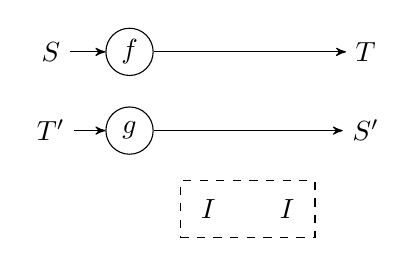
\begin{tikzpicture}
\begin{scope}[on grid]
\node (S) at (0, 0) {$S$};
\node (S') at (4, 0) {$T$};
\node (T) [below = 1 of S] {$T'$};
\node (T') [below = 1 of S'] {$S'$};
\node[vert] (f) [right = 1 of S] {$f$};
\node[vert] (g) [right = 1 of T] {$g$};

\draw[->] (S) -- (f);
\draw[->] (f) -- (S');

\draw[->] (T) -- (g);
\draw[->] (g) -- (T');

\node (I) [below right = 1 and 2 of T] {$I$};
\node (I') [below left = 1 and 1 of T'] {$I$};

\node[draw,dashed,fit=(I) (I'), inner xsep = 4pt] (box) {};
\end{scope}
\end{tikzpicture}
    \qquad \raisebox{1.5cm}{$=$} \qquad
    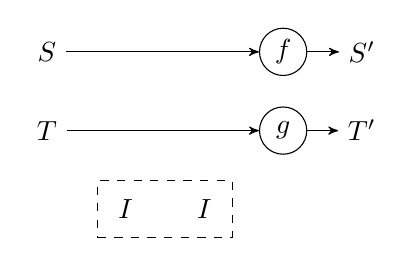
\begin{tikzpicture}
\begin{scope}[on grid]
\node (S) at (0, 0) {$S$};
\node (S') at (4, 0) {$S'$};
\node (T) [below = 1 of S] {$T$};
\node (T') [below = 1 of S'] {$T'$};
\node[vert] (f) [left = 1 of S'] {$f$};
\node[vert] (g) [left = 1 of T'] {$g$};

\draw[->] (S) -- (f);
\draw[->] (f) -- (S');

\draw[->] (T) -- (g);
\draw[->] (g) -- (T');

\node (I) [below right = 1 and 1 of T] {$I$};
\node (I') [below left = 1 and 2 of T'] {$I$};

\node[draw,dashed,fit=(I) (I'), inner xsep = 4pt] (box) {};
\end{scope}
\end{tikzpicture}
  \end{center}
  Symmetry:
  \begin{center}
    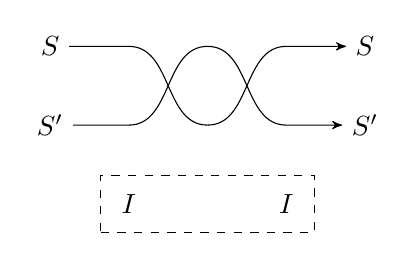
\begin{tikzpicture}
\begin{scope}[on grid]
\node (S) at (0, 0) {$S$};
\node (S2) at (4, 0) {$S$};
\node (S') [below = 1 of S] {$S'$};
\node (S'2) [below = 1 of S2] {$S'$};

\draw[->] (S) -- ++(1,0) to[out = east, in = west] ++(1,-1) to[out = east, in = west] ++ (1,1) -- (S2);
\draw[->] (S') -- ++(1,0) to[out = east, in = west] ++(1,1) to[out = east, in = west] ++ (1,-1) -- (S'2);

\node (I) [below right = 1 and 1 of S'] {$I$};
\node (I') [below left = 1 and 1 of S'2] {$I$};

\node[draw,dashed,fit=(I) (I'), inner xsep = 4pt] (box) {};
\end{scope}
\end{tikzpicture}
    \qquad \raisebox{1.5cm}{$=$} \qquad
    \begin{tikzpicture}
\begin{scope}[on grid]
\node (S) at (0, 0) {$S$};
\node (S2) at (4, 0) {$S$};
\node (S') [below = 1 of S] {$S'$};
\node (S'2) [below = 1 of S2] {$S'$};

\draw[->] (S) -- (S2);
\draw[->] (S') -- (S'2);

\node (I) [below right = 1 and 1 of S'] {$I$};
\node (I') [below left = 1 and 1 of S'2] {$I$};

\node[draw,dashed,fit=(I) (I'), inner xsep = 4pt] (box) {};
\end{scope}
\end{tikzpicture}
  \end{center}
  Monoidality: \todo{there is basically nothing to do in the graphical calculus}

  Note that the diagrams required to commute all terminate with the unit $I$, so in view of Proposition~\ref{prop-costates} we should not be surprised that they correspond to equality of maps in $\C$.
\end{proof}

      %       \todo{They stress about the empty set, have I avoided that issue?}

\begin{proposition}
  The functor $\Optic : \SymmMonCat \to \SymmMonCat$ of Proposition~\ref{prop-optic-functor} has its image in the subcategory $\Tele$.
\end{proposition}
\begin{proof}
  We must show that for a symmetric monoidal functor $F : \C \to \D$, the induced functor $F : \Optic_\C \to \Optic_\D$ is teleological.

  First, $F$ preserves the dualisable morphisms. If $\iota(f, g) : (S, S') \hto (A, A')$,
  \begin{align*}
    F\iota(f, g)
    &= F(\langle \lambda_A^{-1} f, g \lambda_{A'} \rangle) \\
    &= \langle \phi^{-1}_{I,A} (F(\lambda_A^{-1} f)), (F(g \lambda_{A'})) \phi_{I,A'}\rangle \\
    &= \langle \phi^{-1}_{I,A} (F\lambda_A^{-1}) (Ff), (Fg)(F \lambda_{A'}) \phi_{I,A'}\rangle \\
    &= \langle (\phi^{-1}_I \otimes FA) \phi^{-1}_{I,A} (F\lambda_A^{-1}) (Ff), (Fg)(F \lambda_{A'}) \phi_{I,A'} (\phi_I \otimes FA) \rangle \\
    &= \langle \lambda_{FA}^{-1} (Ff), (Fg)\lambda_{FA'} \rangle \\
    &= \iota(Ff, Fg)
  \end{align*}

  And it also preserves the counits:
  \begin{align*}
    F(\varepsilon_{(S, S')})
    &= F(c_{S \otimes S'}) \\
    &= F(\langle \rho_S^{-1}, \rho_{S'} \rangle) \\
    &= \langle \phi^{-1}_{S,I} (F \rho_S^{-1}), (F \rho_{S'}) \phi_{S',I}\rangle \\
    &= \langle (FS \otimes \phi_I^{-1}) \phi^{-1}_{S,I} (F \rho_S^{-1}), (F \rho_{S'}) \phi_{S',I} (FS \otimes \phi_I)\rangle \\
    &= \langle \rho_{FS}^{-1}, \rho_{FS'} \rangle \\
    &= \varepsilon_{(FS, FS')}
  \end{align*}

  \todo{This works fine when $\C$ is not strict}
\end{proof}

      %       \begin{proposition}
      %       Suppose $\langle l, r \rangle : (S, S') \hto (A, A')$ has complement $M$. Then
      %       \begin{align*}
      %       \langle l, r \rangle = (\varepsilon_{(M, I)} \otimes (A, A'))\iota(l, r).
      %     \end{align*}
      %       \end{proposition}
      %       \begin{proof}
      %       First note that because $\C$ is strict monoidal, the counit $\varepsilon_{(M, I)} : (M \otimes I, M \otimes I) = (M, M) \hto (I, I)$ is equal to the connector $c_M : (M, M) \hto (I, I)$.
      %
      %       The claim then holds, as any optic
      %       \begin{center}
      %       \begin{tikzpicture}
\node[vert] (l) at (0, 0) {$l$};
\node[vert] (r) at (4, 0) {$r$};

\node (S) [left of=l] {$S$};
\node (A) [below right = 0.7 and 1 of l] {$A$};
\node (S') [right of=r] {$S'$};
\node (A') [below left = 0.7 and 1 of r] {$A'$};

\draw[->] (S) -- (l);
\draw[->] (l) to[out=south east,in=west] (A);

\draw[<-] (S') -- (r);
\draw[<-] (r) to[out=south west,in=east] (A');

\draw[->] (l) to[rrel, out=north east, in=west] (1,1)
 to +(2,0)
 to[out=east, in=north west] (r)
;

\node[draw,dashed,fit=(A) (A'), inner xsep = 8pt] (box) {};
\end{tikzpicture}
      %       \end{center}
      %       is equal to the composite
      %       \begin{center}
      %       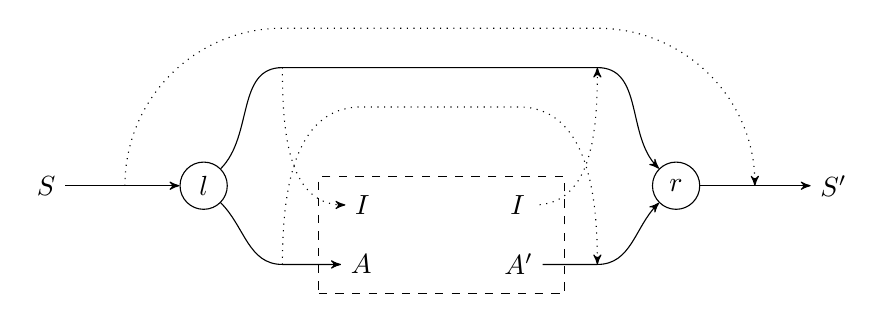
\begin{tikzpicture}
\begin{scope}[on grid]

\node[vert] (l) at (0, 0) {$l$};
\node[vert] (r) at (6, 0) {$r$};

\node (S) [left= 2 of l] {$S$};
\node (A) [below right = 1 and 2 of l] {$A$};
\node (S') [right= 2 of r] {$S'$};
\node (A') [below left = 1 and 2 of r] {$A'$};

\draw[->] (S) -- (l);
\draw[->] (l) 
  to[out=south east,in=west] ($(l) + (1, -1)$)
  to[out=east, in=west] (A);

\draw[<-] (S') -- (r);
\draw[<-] (r) 
  to[out=south west,in=east] ($(r) + (-1, -1)$)
  to[out=west, in=east] (A');

\draw[->] (l) to[out=north east, in=west] ++(1,1.5) coordinate (Mleft) 
 to  ($(r) + (-1, 1.5)$) coordinate (Mright)
 to[out=east, in=north west] (r)
;

\node (I) [below right = 1.5 and 0.8 of Mleft] {$I$};
\node (I') [below left = 1.5 and 0.8 of Mright] {$I$};

\draw[->, dotted] (Mleft) 
  to[out=south, in=west] (I);
\draw[<-, dotted] (Mright) 
  to[out=south, in=east] (I');

\draw[->, dotted]  ($(l) + (-1, 0)$)
 to[out=north, in=west] ++(2,2)
 to[out=east, in=west] ($(r) + (-1, 2)$)
 to[out=east, in=north] ($(r) + (1, 0)$)
;

\draw[->, dotted]  ($(A) + (-1, 0)$)
 to[out=north, in=west] ++(1,2)
 to[out=east, in=west] ($(A') + (0, 2)$)
 to[out=east, in=north] ($(A') + (1, 0)$)
;

%
%\node[vert] (l') at (0, -2) {$l'$};
%\node[vert] (r') at (6, -2) {$r'$};
%
%\node (T) [left of=l'] {$T$};
%\node (B) [below right = 1 and 2 of l'] {$B$};
%\node (T') [right of=r'] {$T'$};
%\node (B') [below left = 1 and 2 of r'] {$B'$};
%
%\draw[->] (T) -- (l');
%\draw[->] (l') to[out=south east,in=west] (B);
%
%\draw[<-] (T') -- (r');
%\draw[<-] (r') to[out=south west,in=east] (B');
%
%\draw[->] (l') 
% to[rrel, out=north east, in=west] (2,2)
% to ++(2,0)
% to[out=east, in=north west] (r')
%;
%

\node[draw,dashed,fit=(A) (A') (I) (I'), inner xsep = 8pt] (box) {};

\end{scope}
\end{tikzpicture}
      %       \end{center}
      %       where we have drawn the normally invisible strings corresponding to the unit $I$.
      %       \end{proof}

\begin{proposition}\label{prop-optic-decompose}
  Suppose $\langle l, r \rangle : (S, S') \hto (A, A')$ has complement $M$. Then
  \begin{align*}
    \langle l, r \rangle = ((A, I) \switched \varepsilon_{(M, I)} \switched (I, A'))(j(s_{M,A}l) \switched j(rs_{A',M})^*)
  \end{align*}
  where $j : \C \to \Optic_\C$ is the functor $j(A) := \iota(A, I)$.
  \todo{The symmetries could have been avoided in the above expression if the Optic category had been defined with the tensor in the opposite order!}
\end{proposition}
\begin{proof}
  First note that because $\C$ is strict monoidal, the counit $\varepsilon_{(M, I)} : (M \otimes I, M \otimes I) = (M, M) \hto (I, I)$ is equal to the connector $c_M : (M, M) \hto (I, I)$.

  Then, up to strictness of the monoidal unit, we are composing the two optics
  \begin{center}
    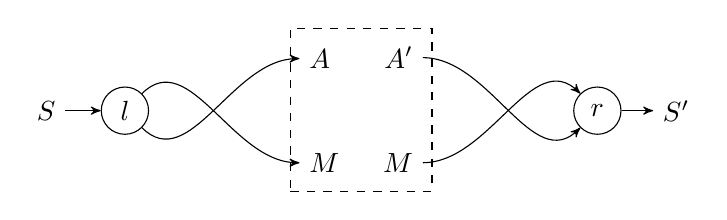
\begin{tikzpicture}

\node (l) [vert] at (0, 0) {$l$};
\node (S) [left of=l] {$S$};
\node (A) [above right = 0.2 and 2 of l] {$A$};
\node (M) [below right = 0.2 and 2 of l] {$M$};

\node (r) [vert] at (6, 0) {$r$};
\node (S') [right of=r] {$S'$};
\node (A') [above left = 0.2 and 2 of r] {$A'$};
\node (M') [below left = 0.2 and 2 of r] {$M$};

\draw[->] (S) -- (l);
\draw[->] (r) -- (S');

\draw[->] (l) to[out=south east, in=west] (A);
\draw[->] (l) to[out=north east, in=west] (M);

\draw[<-] (r) to[out=south west, in=east] (A');
\draw[<-] (r) to[out=north west, in=east] (M');

\node[draw,dashed,fit=(A) (A') (M) (M')] (box) {};
\end{tikzpicture}
  \end{center}
  and
  \begin{center}
    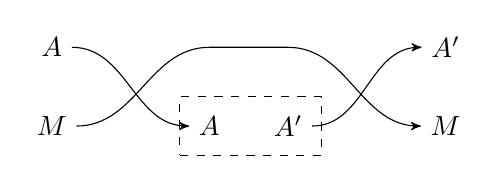
\begin{tikzpicture}
\begin{scope}[on grid]

\node (A) at (0, 0) {$A$};
\node (M) [below = 1 of A] {$M$};
\node (A') at (5, 0) {$A'$};
\node (M') [below = 1 of A'] {$M$};

\node (Aout) [below right = 1 and 2 of A] {$A$};
\node (A'out) [below left= 1 and 2 of A'] {$A'$};

\draw[->] (A) to[out=east, in=west] (Aout);
\draw[<-] (A') to[out=west, in=east] (A'out);

\draw[->] (M) to[out=east, in=west] ($(Aout) + (0,1)$)
to[out=east, in=west] ($(A'out) + (0,1)$)
to[out=east, in=west] (M');

\node[draw,dashed,fit=(Aout) (A'out) ] (box) {};

\end{scope}
\end{tikzpicture}
  \end{center}
  so the two pairs of twists cancel, and we are left exactly with the diagram for $\langle l, r \rangle$.
\end{proof}

\begin{theorem}
  \label{optic-is-free-teleological-cat}
  Suppose $\C$ is a strict symmetric monoidal category and $\T$ is a teleological category. For all symmetric monoidal functors $F : \C \to \T_d$, there exists a teleological functor $K : \Optic_\C \to \T$, unique up to isomorphism, such that $Kj \cong F$.
  % $\Optic$ is left adjoint to $(-)_d$, so $\Optic_\C$ is the free teleological category on a category of dualisable morphisms $\C$.
\end{theorem}
\begin{proof}
  On objects, define $K(S, S') = FS \otimes (FS')^*$. Suppose $\langle l, r \rangle : (S, S') \hto (A, A')$ is an optic. By the previous Proposition,
  \begin{align*}
    \langle l, r \rangle = ((A, I) \switched \varepsilon_{(M, I)} \switched (I, A'))(j(s_{M,A}l) \switched j(rs_{M,A'})^*)
  \end{align*}
  But now, in order for $K$ to be a teleological functor with $Kj \cong F$, each piece of this expression must be preserved by $K$, so we are forced to define:
  \begin{align*}
    K\langle l, r \rangle = (FA \otimes \varepsilon_{FM} \otimes (FA')^*)(F(s_{M,A}l) \otimes (F(rs_{A', M}))^* )
  \end{align*}

  We must show that this is well defined. Suppose we have two lenses related by the coend relation:
  \begin{align*}
    \langle (f \otimes A) l, r \rangle = \langle l, r (f \otimes A') \rangle
  \end{align*}
  Then: \todo{maybe do as string diagram}
  \begin{align*}
    K\langle (f \otimes A) l, r \rangle
    &= (FA \otimes \varepsilon_{FM} \otimes (FA')^*)(F(s_{M,A}(f \otimes A)l) \otimes (F(rs_{A',M}))^* ) \\
    &= (FA \otimes \varepsilon_{FM} \otimes (FA')^*)(F((A \otimes f)s_{N,A}l) \otimes (F(rs_{A',M}))^* ) \\
    % &= (FA \otimes \varepsilon_{FM} \otimes (FA')^*)(FA \otimes Ff \otimes FM \otimes FA')(F(s_{N,A}l) \otimes (F(rs_{A',M}))^* ) \\
    &= (FA \otimes (\varepsilon_{FM} (Ff \otimes FM)) \otimes (FA')^*)(F(s_{N,A}l) \otimes (F(rs_{A',M}))^* ) \\
    &= (FA \otimes (\varepsilon_{FN} (FN \otimes (Ff)^*)) \otimes (FA')^*)(F(s_{N,A}l) \otimes (F(rs_{A',M}))^* ) \\
    &= (FA \otimes \varepsilon_{FN} \otimes (FA')^*)(F(s_{N,A}l) \otimes (F(rs_{A',M}(A' \otimes f)))^* ) \\
    &= (FA \otimes \varepsilon_{FN} \otimes (FA')^*)(F(s_{N,A}l) \otimes (F(r(f \otimes A')s_{A',N}))^* ) \\
    &= K\langle  l, r (f \otimes A') \rangle
  \end{align*}
  \todo{functoriality} \todo{monoidal} \todo{preserves dualisable morphisms} \todo{preserves counit}
\end{proof}

\subsection{Optics for a Monoidal Action}

To capture the \texttt{Iso}s, \texttt{Traversal}s and \texttt{Setter}s of the Haskell \texttt{lens} library (see~\ref{lawful-examples}), we generalise to the case of a monoidal action of one category on another.

\begin{definition}
  Let $\C$ be a category and $(\M, \otimes, I)$ a monoidal category. An \emph{action of $\M$ on $\C$} is a strong monoidal functor $a : \M \to [\C, \C]$. The action of an object $M \in \M$ on $A \in \C$ is written $MA$.
\end{definition}

Given such an action, we define
\begin{align*}
  \Optic_\M((S, S'), (A, A')) := \int^{M \in \C} \C(S, MA) \times \C(MA', S')
\end{align*}

\begin{proposition}
  We have a category $\Optic_\M$ and a functor $\iota : \C \times \C^\op \to \Optic_\M$. \qed
\end{proposition}

\begin{proposition}\label{prop-change-of-action}
  Suppose $\C$ and $\D$ are categories acted on by $\M$ and $\mathcal{N}$ respectively. If $F : \C \to \D$ is a functor that commutes with the actions, then there is an induced functor $\Optic(F) : \Optic_\M \to \Optic_\N$.
\end{proposition}
\begin{proof}
  Analogous to Proposition~\ref{prop-change-of-action-monoidal}
\end{proof}

For the remainder of the paper we work in this slightly more general setting.

\section{Lawful Optics}
\todo{intro}
\todo{Here I am using ; to mean composition in diagrammatic order, I need to make a final decision on which to use}

\begin{remark}
  In this section we will focus only on optics of the form $p : (S,S) \hto (A, A)$. For brevity we will write $\Optic_\M((S, S), (A, A))$ as $\Optic_\M(S, A)$ and $p : (S, S) \hto (A, A)$ as $p : S \hto A$.
\end{remark}

\todo{In this section I am using semicolon to mean composition in diagrammatic order. Should I also switch the comma in $\langle l, r \rangle$ to be a $\mid$?}

For a fixed $M \in \M$, there is a map $\C(S, M A) \times \C(M A, S) \to \C(S, S)$ given by composition. This induces a map $\outside : \Optic_\M(S, A) \to \C(S, S)$, given equationally by $\outside(\langle l, r \rangle) = l ; r$

There are also maps two maps
\begin{align*}
  \once, \twice : \Optic_\M(S, A) \to \int^{M_1, M_2 \in \M} \C(S, M_1 A) \times \C(M_1 A, M_2 A) \times \C(M_2 A, S)
\end{align*}
defined by
\begin{align*}
  \once(\langle l, r \rangle) &= \langle l, \id_{MA}, r \rangle \\
  \twice(\langle l, r \rangle) &= \langle l, r;l, r \rangle
\end{align*}

\begin{definition}
  An optic $p : S \hto A$ is \emph{lawful} if
  \begin{align*}
    \outside(p) &= \id_S \\
    \once(p) &= \twice(p)
  \end{align*}
\end{definition}

We will see that in all the standard examples of optics, this specialises to the expected laws for that type of optic.

\begin{remark}
  Jeremy Gibbons notes (originally in the case of ordinary lenses) that the first law is equivalent to requiring that $p$ composed with the connector $c_A$ is equal to the connector $c_S$. This is an appealing description from a string diagram standpoint, but I do not know if there is a similar description for the second law. \todo{Something to do with embedding $\Optic_\C$ into a compact closed category then using the unit to compose the lenses vertically? Should I draw a picture of this?}
\end{remark}

\begin{proposition}
  There is an subcategory $\Lawful_\M$ of $\Optic_\M$ given by objects of the form $(S, S)$ and lawful optics between them.
\end{proposition}
\begin{proof}
  The identity optic $\iota(\id_S, \id_S)$ is lawful:
  \begin{align*}
    \outside(\langle \lambda^{-1}_S, \lambda_{S} \rangle) &= \lambda_{S} \lambda^{-1}_S = \id_S \\
    \intertext{and}
    \once(\langle \lambda^{-1}_S, \lambda_{S} \rangle)
                                                          &= \langle \lambda^{-1}_S, \id_{IA}, \lambda_{S} \rangle \\
                                                          &= \langle \lambda^{-1}_S, \lambda_{S};\lambda^{-1}_S , \lambda_{S} \rangle \\
                                                          &= \twice(\langle \lambda^{-1}_S, \lambda_{S} \rangle)
  \end{align*}

  Suppose we have two lawful optics $\langle l, r \rangle : R \hto S$ and $\langle l', r' \rangle : S \hto A$, where $l : R \to MS$ and $l' : S \to NA$. We must show that $\langle (Ml')l, r (Mr')  \rangle$ is also a lawful optic. The first equation is straightforward:
  \begin{align*}
    \outside(\langle l; (Ml'),(Mr') ; r   \rangle)
    &= l ; Ml' ; Mr' ; r \\
    &= l ; M(l'r') ; r \\
    &= l ; M\id_{NA} ; r \\
    &= l ; r \\
    &= \id_{MNA}
  \end{align*}

  For the second, we must show
  \[ \langle l;(Ml'), (Mr'); r;l;(Ml') , (Mr') ; r  \rangle = \langle l;(Ml'), \id_{MNA} , (Mr') ; r  \rangle. \]

  We do this by showing that, in some sense, the expressions in the above equation respect the coend relations defining the codomains of $\once(\langle l, r \rangle)$ and $\once(\langle l', r' \rangle)$.

  So consider the generating relation $\langle l;\phi_S, c, r \rangle = \langle l, \phi_S ; c, r \rangle$ in \[\int^{M_1, M_2 \in \M} \C(R, M_1 S) \times \C(M_1 S, M_2 S) \times \C(M_2 S, R).\]
  This implies that
  \begin{align*}
    \langle l;\phi_S;(Ml'), (Mr'); c ;(Ml') , (Mr') ; r \rangle
    &= \langle l;(Ml');\phi_{NA}, (Mr'); c ;(Ml') , (Mr') ; r \rangle && \text{(functoriality)} \\
    &= \langle l;(Ml'), \phi_{NA};(Mr'); c ;(Ml') , (Mr') ; r \rangle && \text{(coend relation)} \\
    &= \langle l;(Ml'), (Mr');\phi_{S}; c ;(Ml') , (Mr') ; r \rangle && \text{(functoriality)}
  \end{align*}
  And similarly for the other generating relation, $\langle l, c;\phi_S, r \rangle = \langle l,  c, \phi_S; r \rangle$.

  Therefore, the chain of relations proving $\langle l, r;l, r \rangle = \langle l, \id_{MA}, r \rangle$ can be replicated to show
  \begin{align*}
    \langle l;(Ml'), (Mr');r;l;(Ml') , (Mr') ; r \rangle &= \langle l;(Ml'), (Mr');\id_{MA};(Ml') , (Mr') ; r \rangle,
  \end{align*}
  which is equal to $\langle l;(Ml'), M(r'l'), (Mr') ; r \rangle$.

  Similarly, a generating relation $\langle l';\psi_A, c', r' \rangle = \langle l', \psi_A ; c', r' \rangle$ in \[\int^{N_1, N_2 \in \M} \C(S, N_1 A) \times \C(N_1 A, N_2 A) \times \C(M_2 A, S)\]
  implies that
  \begin{align*}
    \langle l;M(l';\psi_A), Mc', (Mr') ; r \rangle
    &= \langle l;Ml';M\psi_A, Mc', (Mr') ; r \rangle \\
    &= \langle l;Ml', M\psi_A ; Mc', (Mr') ; r \rangle \\
    &= \langle l;Ml', M(\psi_A;c'), (Mr') ; r \rangle
  \end{align*}
  So again we can replicate the chain of relations proving $\langle l', r';l', r' \rangle = \langle l', \id_{MA}, r' \rangle$ to show that
  \[\langle l;(Ml'), M(r'l'), (Mr') ; r \rangle = \langle l;(Ml'), \id_{MNA}, (Mr') ; r \rangle \]

  We conclude that composition preserves lawfulness, so $\Lawful_\M$ is indeed a subcategory of $\Optic_\M$.

  \todo{There is probably a more conceptual way to do this}
\end{proof}

\begin{proposition}
  If $F : \C \to \D$ is a functor that commutes with the monoidal actions on $\C$ and $\D$, then $\Optic(F) : \Optic_\M \to \Optic_\N$ restricts to a functor $\Lawful_\M \to \Lawful_\N$.
\end{proposition}
\begin{proof}
  If $p = \langle l, r \rangle$ is lawful,
\end{proof}

The requirement that $\once(p) = \twice(p)$ is mysterious, but there are sufficient conditions that are easier to verify.

\begin{proposition}
  Let $\langle l, r \rangle : S \hto A$ be an optic. If $l;r = \id_S$ and $r;l = \phi A$ for some $\phi : M \to M$ in $\M$, then $\langle l, r \rangle$ is a lawful optic.
\end{proposition}
\begin{proof}
  The $\outside(\langle l, r \rangle) = l;r = \id_S$ is exactly the first condition. And for the second, we verify:
  \begin{align*}
    \twice(\langle l, r \rangle)
    &= \langle l, r;l, r \rangle \\
    &= \langle l, \phi A, r \rangle && \text{($r;l = \phi A$)}\\
    &= \langle l (\phi A), \id_{MA}, r \rangle && \text{(coend relation)} \\
    &= \langle l;r;l, \id_{MA}, r \rangle && \text{($r;l = \phi A$ again)}\\
    &= \langle l, \id_{MA}, r \rangle  && \text{($l;r = \id_S$)}\\
    &= \once(\langle l, r \rangle)
  \end{align*}
\end{proof}

\begin{remark}
  Even if $r;l = \phi A$ for some $\phi$, the same is not necessarily true of any other representative of the same optic.
\end{remark}

Let $\inside : \Optic_\M(S, A) \to \int^{M \in \M} \C(M A, M A)$ be the map induced by $\inside(\langle l, r \rangle) = \langle r ; l \rangle$. We might ask that instead of requiring $r;l = \phi A$ exactly, we have $\langle r ; l \rangle = \langle \phi A \rangle$ in $\int^{M \in \M} \C(M A, M A)$. In fact, this is equivalent:

\begin{proposition}\label{prop-onthenose}
  Suppose $p : S \hto A$ satisfies $\outside(p) = \id_S$ and $\inside(p) = \langle \phi A \rangle$. Then there exists a representative $\langle l, r \rangle$ such that $l ; r = \psi A$ on the nose for some (possibly different) $\psi : M \to M$.
\end{proposition}
\begin{proof}
  \todo{Go through this proof for formatting again.}

  The coend relation in $\int^{M \in \M} \C(M A, M A)$ states that two morphisms $f : M A \to M A$ and $g : N A \to N A$ are identified when there exists a $k : N A \to M A$ and morphism $\phi : M \to N$ such that
  \[
    \begin{tikzcd}
      M A \ar[r, "\phi_A"] \ar[d, "f", swap] & N A \ar[d, "g"] \ar[dl, "k"] \\
      M A \ar[r, "\phi_A", swap] & N A
    \end{tikzcd}
  \]
  commutes. This gives a binary relation $f \rightsquigarrow g$ that is not likely to be symmetric or transitive in general. The coend is obtained by identifying all morphisms related in this way, $\langle f \rangle = \langle g \rangle$ iff there exists a zigzag $f = u_1 \leftrightsquigarrow u_2 \leftrightsquigarrow \dots  \leftrightsquigarrow u_{n-1} \leftrightsquigarrow u_n = g$ where the relation may apply in either direction.

  Note that if $f \rightsquigarrow g$ then $ff \rightsquigarrow gg$: this is clear by stacking the above diagram, and then taking $k' = fk = kg$. This argument can be repeated to show that $f^n \rightsquigarrow g^n$ for any $n$.

  Similarly two representatives $\langle l, r \rangle : S \hto A$ and $\langle l', r' \rangle : S \hto A$ with complements $M$ and $N$ respectively are identified when there exists a $\phi : M \to N$ such that
  \[
    \begin{tikzcd}
      M A \ar[r, "\phi_A"] \ar[d, "r", swap] & N A \ar[d, "r'"] \\
      S \ar[r, equal] \ar[d, "l", swap] & S \ar[d, "l'"]  \\
      MA \ar[r, "\phi_A"] & N A
    \end{tikzcd}
  \]
  commutes.

  Now suppose $p = \langle l, r \rangle : S \hto A$ is a lawful optic, so $rl = \id_S$ and $\langle lr \rangle = \langle \psi A\rangle$. There therefore must exist a finite chain of relations $lr = u_1 \leftrightsquigarrow \dots \leftrightsquigarrow u_n = \psi A$.
  Supposing that the first relation faces rightwards, we have a diagram:
  \[
    \begin{tikzcd}
      M A \ar[r, "\phi_A"] \ar[d, "r", swap] & N A \ar[dd, "u_2"] \ar[ddl, "k"] \\
      S \ar[d,"l",swap] & \\
      M A \ar[r, "\phi_A", swap] & N A
    \end{tikzcd}
  \]
  Note that $r = rlr = rk\phi_A$. We therefore have the commutative diagram
  \[
    \begin{tikzcd}
      M A \ar[r, "\phi_A"] \ar[d, "r", swap] & N A \ar[d, "rk"] \\
      S \ar[r, equal] \ar[d, "l", swap] & S \ar[d, "\phi_Al"] \\
      MA \ar[r, "\phi_A", swap] & N A
    \end{tikzcd}
  \]
  Define $l' = \phi_A l$ and $r' = rk$. The above diagram is a witness that $\langle l, r \rangle = \langle l', r' \rangle$ as an optic $S \hto A$.

  The composite $l'r'$ is:
  \begin{align*}
    l'r' &= \phi_A l r k \\
         &= \phi_A k \phi_A k \\
         &= u_2^2
  \end{align*}

  A symmetric argument shows that if instead the relation faces leftward, so $lr \leftsquigarrow g$, there exists $l'$ and $r'$ so that $\langle l, r \rangle = \langle l', r' \rangle$ and $l'r' = u_2^2$.

  We can now inductively apply the above argument to the shorter chain \[l'r' = u_1^2 \leftrightsquigarrow \dots \leftrightsquigarrow u_n^2 \leftrightsquigarrow (\psi A)^2 = \psi^2 A,\] obtained by squaring each morphism in the original chain, until we are left with a representative $\langle l^*, r^* \rangle$ such that $l^*r^* = \psi^N A$, for some $N>0$. This pair $\langle l^*, r^* \rangle$ is the required representative.
\end{proof}

The above argument has a similar form to some that appear in \cite{OnTheTrace}, which considered (among other things) coends of the form $\int^{c \in \C} \C(c, Fc)$ for an endofunctor $F : \C \to \C$.

Finally, lawfulness is preserved by the change-of-action functors of Proposition \ref{prop-change-of-action}.

\section{Examples}
\label{lawful-examples}

The general pattern is as follows. Once we choose a particular monoidal action $\M \to [\C, \C]$, we find an isomorphism between the set of optics $(S, S') \hto (A, A')$ and a set $\mathbb{O}((S, S'), (A, A'))$ that is easier to describe. Ideally, we then find a similar description $\mathbb{D}(S, A)$ for the set \[ \int^{M_1, M_2 \in \M} \C(S, M_1 A) \times \C(M_1 A, M_2 A) \times \C(M_2 A, S)\] appearing in the definition of a lawful optic. We can then ``read off'' what conditions on an element of $\mathbb{O}((S, S), (A, A))$ are needed to ensure that the corresponding element of $\Optic_\M(S, A)$ is lawful.

\todo{As we get higher up in the hierarchy, the `ad-hoc' laws get closer to being the same as the coend laws}

\subsection{Lenses}

Lenses form the ur-example of a category of optics.

\begin{definition}
  Suppose $\C$ has finite products, and let $\C$ act on itself via the bifunctor $\times : \C \times \C \to \C$. The \emph{category of lenses} $\Lens$ is the category of lawful optics with respect to this action: $\Lens = \Lawful_\times$.
\end{definition}

The optics for this action correspond exactly to pairs of $\fget$ and $\fput$ functions.
\begin{align*}
  \Optic_\times((S, S'), (A, A')) &= \int^{M \in \C} \C(S, M \times A) \times \C(M \times A', S') \\
                                  &\cong \int^{M \in \C} \C(S, M) \times \C(S, A) \times \C(M \times A', S') && \text{(universal property of product)} \\
                                  &\cong \C(S, A) \times \C(S \times A', S') && \text{(co-Yoneda)} \\
                                  &=: \mathbb{O}((S, S'), (A, A'))
\end{align*}

Explicitly this isomorphism states that, given an optic $\langle l, r \rangle : (S, S') \hto (A, A')$, the corresponding element of $\mathbb{O}((S, S'), (A, A'))$ is the pair $(\fget, \fput)$, where $\fget = \pi_2 l$ and $\fput = r (\pi_1 l \times A)$. In the other direction, given $(\fget, \fput)$, the corresponding optic has representative $\langle [\id_S, \fget],  \fput \rangle$.

\begin{remark}\label{lens-iota-not-faithful}
  For the category of sets, the functor $\iota(-, -) : \Set \times \Set^\op \to \Optic_\times$ is not faithful. The problem is the empty set: the functor $0 \times (-)$ is not faithful. Any pair of maps $f : 0 \to A$, $g : A' \to S'$ yield equivalent optics $\iota(f, g)$, as the corresponding $\fget$ and $\fput$ functions must be the unique maps from $0$.
\end{remark}

\begin{remark}
  In the case that $\C$ is cartesian closed, $\Optic_\times$ is monoidal closed via the astonishing formula
  \begin{align*}
    [(S, S'), (A, A')] := (\homC(S, A) \times \homC(S \times A', S'), \, S \times A')
  \end{align*}
  where $\homC(-, -)$ denotes the internal hom. For a proof see~\cite[Section 1.2]{DialecticaCategories}. This cannot be extended to non-cartesian closed categories, the isomorphism
  \begin{align*}
    \Optic_\times((S, S') \otimes (T, T'), (A, A')) \cong \Optic_\times((S, S'),  [(T, T'), (A, A')])
  \end{align*}
  uses the diagonal maps of $\C$ in an essential way.
\end{remark}

We now discuss lawful lenses.

\begin{proposition}\label{prop-OpticImpliesLensLaws}
  A lens $p : S \hto A$ is a lawful lens in our sense, i.e.\ that $\outside(p) = \id_S$ and $\once(p) = \twice(p)$, if and only if the corresponding $\fput$ and $\fget$ for this lens obey the three lens laws.
\end{proposition}
\begin{proof}
  We begin by giving
  \[ \int^{M_1, M_2 \in \C} \C(S, M_1 \times A) \times \C(M_1 \times A, M_2 \times A) \times \C(M_2 \times A, S)\]
  the same treatment as $\Optic_\times(S, A)$. By the same sorts of arguments as above \todo{is this worth writing out?}, this is isomorphic to
  \[\mathbb{D}(S, A) := \C(S, A) \times \C(S \times A, A) \times \C(S \times A \times A, S)\]
  with the isomorphism given by
  \begin{align*}
    \Phi(\langle l, c, r \rangle) = (&\pi_2 l, \\
                                     &\pi_2 c (\pi_1 l \times A), \\
                                     &r(\pi_1 c (\pi_1 l \times A) \times A))
  \end{align*}
  Now suppose we are given a lens $(\fget, \fput)$, which in coend form is $\langle [\id_S, \fget],  \fput \rangle$. Evaluating $\outside$ on this gives:
  \begin{align*}
    \outside(\langle [\id_S, \fget],  \fput \rangle) = \fput [\id_S, \fget]
  \end{align*}
  so requiring $\outside(p) = \id_S$ is precisely the $\fget\fput$ law.

  We now have to slog through evaluating $\Phi(\once(p))$ and $\Phi(\twice(p))$.
  \begin{alignat*}{3}
    \Phi(\once(\langle [\id_S, \fget],  \fput \rangle)) &=
    \Phi(&&\langle [\id_S, \fget], \id_{S \times A}, \fput \rangle) \\
    &= (&&\pi_2 [\id_S, \fget], \\
    &&&\pi_2 \id_{S \times A} (\pi_1 [\id_S, \fget] \times A), \\
    &&& \fput (\pi_1 \id_{S \times A} (\pi_1 [\id_S, \fget] \times A) \times A) \quad) \\
    %
    &= (&&\fget, \\
    &&& \pi_2, \\
    &&& \fput \pi_{1,3} \quad) \\
    %%%%
    %%%%
    \Phi(\twice(\langle [\id_S, \fget],  \fput \rangle)) &=
    \Phi(&&\langle [\id_S, \fget], [\id_S, \fget]\fput, \fput \rangle) \\
    &= (&&\pi_2 [\id_S, \fget], \\
    &&&\pi_2 [\id_S, \fget]\fput (\pi_1 [\id_S, \fget] \times A), \\
    &&& \fput (\pi_1 [\id_S, \fget]\fput (\pi_1 [\id_S, \fget] \times A) \times A)) \quad) \\
    %
    &= (&&\fget, \\
    &&& \fget \; \fput (\id_S \times A), \\
    &&& \fput (\fput (\id_S \times A) \times A) \quad) \\
    %
    &= (&&\fget, \\
    &&& \fget \; \fput, \\
    &&& \fput (\fput \times A) \quad)
  \end{alignat*}
  So checking componentwise, $\Phi(\once(p))$ being equal to $\Phi(\twice(p))$ is exactly equivalent to the $\fput\fget$ and $\fput\fput$ laws holding.
\end{proof}

\todo{This last proposition should probably be deleted now}

In favourable conditions, we can upgrade this result to show that the existence of a lens $S \hto A$ implies that $S \cong C \times A$ for some $C$. This is a generalised from the argument given in~\cite[Corollary 13]{AlgebrasAndUpdateStrategies} for $\Set$.

\begin{proposition}
  Suppose $\C$ has pullbacks and that there is a morphism $x : 1 \to A$. If $\fget : S \to A$ and $\fput : S \times A \to S$ satisfy the three lens laws then there exists $C \in \C$ with $S \cong C \times A$.
\end{proposition}
\begin{proof}
  Set $C$ to be the pullback of $\fget$ along $x$, so there is a map $i : C \to S$ with $\fget \, i = x !_C$. There is also a map $j : S \to C$ induced by the following diagram:
  \[
    \begin{tikzcd}
      S \ar[ddr, bend right = 20] \ar[dr, "j", dashed] \ar[r, "{[\id_S, x !_S]}"] & S \times A \ar[dr, "\fput"] & \\
      & C \ar[r, "i"] \ar[d] \arrow[dr, phantom, "\lrcorner", very near start] & S \ar[d, "\fget"] \\
      & 1\ar[r, "x", swap] & A
    \end{tikzcd}
  \]
  which commutes by the $\fput\fget$ law. Note that $ji = \id_C$ by the universal property of pullbacks. The claim is that $\fput (i \times A) : C \times A \to S$ and $[j,\fget] : S \to C \times A$ are mutual inverses. This is easily checked:
  \begin{align*}
    \fput (i \times A)[j,\fget] &= \fput [ij,\fget] \\
                                &= \fput [\fput [\id_S, x!_S],\fget] && \text{(by definition of $j$)} \\
                                &= \fput [\id_S,\fget] && \text{(by $\fput\fput$)} \\
                                &= \id_S && \text{(by $\fget\fput$)}
                                            \intertext{and}
                                            [j,\fget]\fput (i \times A) &= [j\fput (i \times A),\fget\,\fput (i \times A)] && \text{(by universal property of product)} \\
                                &= [j\fput (i \times A), \pi_2 (i \times A)] && \text{(by $\fput\fget$)} \\
                                &= [j\fput (i \times A), \pi_2] && \\
                                &= [jij\fput (i \times A), \pi_2] && \\
                                &= [j\fput [\id_S,x !_S] \fput (i \times A), \pi_2] && \\
                                &= [j\fput [\id_S, x !_S] \pi_1 (i \times A), \pi_2] && \text{(by $\fput\fput$ \todo{todo: detail})}\\
                                &= [jij \pi_1 (i \times A), \pi_2] && \\
                                &= [jiji \pi_1, \pi_2] && \\
                                &= [\pi_1, \pi_2] && \\
                                &= \id_{C \times A}
  \end{align*}

  Additionally, the commutative diagram
  \[
    \begin{tikzcd}
      C \times A \ar[r, "i \times A"] \ar[d, "\fput (i \times A)", swap] & S \times A \ar[d, "\fput"] \\
      S \ar[r, equal] \ar[d, "{[j,\fget]}", swap] & S \ar[d, "{[\id_S, \fget]}"]  \\
      C \times A \ar[r, "i \times A", swap] & S \times A
    \end{tikzcd}
  \]
  is a witness that $\langle \fput (i \times A), [j,\fget] \rangle = \langle \fput, [\id_S, \fget] \rangle$ as elements of $\Optic_\M(S, A)$.
\end{proof}

\todo{There may be something generalisable here with ``monoidal factorisation systems''}

\subsection{Linear Lenses}
\newcommand{\ev}{\mathsf{ev}}
\newcommand{\coev}{\mathsf{coev}}

If $\C$ is closed monoidal, we can use a similar trick to eliminate the coends.

\begin{align*}
  \Optic_\otimes((S, S'), (A, A')) &= \int^{M \in \C} \C(S, M \otimes A) \times \C(M \otimes A', S') \\
                                   &\cong \int^{M \in \C} \C(S, M \otimes A) \times \C(M, \homC(A',S')) \\
                                   &\cong \C(S, \homC(A',S') \otimes A) \\
                                   &=: \mathbb{O}((S, S'), (A, A'))
\end{align*}
where $\homC(A', S')$ denotes the internal hom. If $\C$ is cartesian, this is of course isomorphic to the pair of maps discussed in the previous section.

For an optic, the corresponding element of $\mathbb{O}((S, S'), (A, A'))$ will be called $\funzip$. The above isomorphism sends $\funzip$ to the element $\langle \funzip , \ev_{A', S'} \rangle$, where $\ev_{A', S'} : \homC(A',S') \otimes A' \to S'$ is the evaluation map. In the other direction, given $\langle l, r \rangle$ we have $\funzip = (\tilde r \otimes A)l$ where $\tilde r : M \to \homC(A', S')$ denotes the transpose of $r$.

We cannot possibly use the three $\fput$/$\fget$ style lens laws in this setting as we lack projections, but using the same techniques as for cartesian lenses above we can devise some new ones:

\begin{proposition}
  A linear lens $p : S \hto A$ is lawful iff the following two laws for $\funzip$ hold:
  \begin{align*}
    \ev_{A, S} \; \funzip &= \id_S && \textsc{(Rezip)} \\
    (\coev_{\homC(A, S), A} \otimes A)\funzip &= ((\funzip \circ -) \otimes A)\funzip && \textsc{(ZipZip)}
  \end{align*}
  where \[ \funzip \circ - : \homC(A, S) \to \homC(A, \homC(A, S) \otimes A) \] denotes the internal composition. \todo{I obviously need better names for the laws}
\end{proposition}
\begin{proof}
  We have an isomorphism:
  \begin{align*}
    & \int^{M_1, M_2 \in \C} \C(S, M_1 \otimes A) \times \C(M_1 \otimes A, M_2 \otimes A) \times \C(M_2 \otimes A, S) \\
    &\cong \int^{M_1, M_2 \in \C} \C(S, M_1 \otimes A) \times \C(M_1, \homC(A, M_2 \otimes A)) \times \C(M_2, \homC(A, S)) \\
    &\cong \int^{M_1 \in \C} \C(S, M_1 \otimes A) \times \C(M_1, \homC(A, \homC(A, S) \otimes A)) \\
    &\cong \C(S, \homC(A, \homC(A, S) \otimes A) \otimes A)
  \end{align*}
  which evaluated on an element $\langle l, c, r \rangle$ is given by
  \begin{align*}
    \Phi(\langle l, c, r \rangle) &= (\widetilde{(\tilde{r} \otimes A)c} \otimes A)l
  \end{align*}
  Now suppose we are given an optic $p$ with corresponding element of $\mathbb{O}(S, A)$ is $\funzip$. Then $\outside(\langle \funzip , \ev_{A, S} \rangle) = \ev_{A, S} \; \funzip$, giving the first law.

  Now we evaluate $\Phi(\once(p))$ and $\Phi(\twice(p))$.
  \begin{align*}
    \Phi(\once(\langle \funzip , \ev_{A, S} \rangle))
    &= \Phi(\langle \funzip , \id_{\homC(A,S) \otimes A}, \ev_{A, S} \rangle) \\
    &= (\widetilde{(\tilde{\ev_{A, S}} \otimes A)\id_{\homC(A,S) \otimes A}} \otimes A)\funzip \\
    &= (\coev_{\homC(A, S), A} \otimes A)\funzip \\
    \Phi(\twice(\langle \funzip , \ev_{A, S} \rangle))
    &= \Phi(\langle \funzip , \funzip \; \ev_{A, S}, \ev_{A, S} \rangle) \\
    &= (\widetilde{(\tilde{\ev_{A, S}} \otimes A)(\funzip \; \ev_{A, S})} \otimes A)\funzip \\
    &= (\widetilde{(\funzip \; \ev_{A, S})} \otimes A)\funzip \\
    &= ((\funzip \circ -) \otimes A)\funzip
  \end{align*}
  \todo{Fix those overtildes}
  So indeed the optic is lawful iff $(\coev_{\homC(A, S), A} \otimes A)\funzip = ((\funzip \circ -) \otimes A)\funzip$.
\end{proof}

\todo{The use of lenses in a language with linear types seems worth exploring!}

\subsection{``Achromatic'' Lenses}
\todo{http://oleg.fi/gists/posts/2018-03-28-achromatic-lens.html}

Suppose $\C$ is cartesian closed and has finite coproducts. Then $\C$ acts on itself via $M \cdot A = (M \sqcup 1) \times A$.
\begin{align*}
  \Optic((S, S'), (A, A'))
  &= \int^{M \in \C} \C(S, M \cdot A) \times \C(M \cdot A', S') \\
  &= \int^{M \in \C} \C(S, (M \sqcup 1) \times A) \times \C((M \sqcup 1) \times A', S') \\
  &\cong \int^{M \in \C} \C(S, (M \sqcup 1) \times A) \times \C((M \times A') \sqcup A', S') \\
  &\cong \int^{M \in \C} \C(S, (M \sqcup 1) \times A) \times \C(M \times A', S') \times \C(A', S') \\
  &\cong \int^{M \in \C} \C(S, (M \sqcup 1) \times A) \times \C(M, \homC(A', S')) \times \C(A', S') \\
  &\cong \C(S, (\homC(A', S') \sqcup 1) \times A) \times \C(A', S') \\
  &\cong \C(S, \homC(A', S') \sqcup 1) \times \C(S, A) \times \C(A', S') \\
\end{align*}

\begin{remark}
  Equivalently, we could let $\M$ be the category of pointed objects of $\C$ and pointed maps between them.
\end{remark}

\todo{Is it worth working the laws out?}

\subsection{Prisms}
Prisms are dual to lenses:

\begin{definition}
  Suppose $\C$ has finite coproducts, and let $\C$ act on itself via the bifunctor $\sqcup : \C \times \C \to \C$. The \emph{category of prisms} is the category of lawful optics with respect to this action: $\Prism = \Lawful_\sqcup$.
\end{definition}

Just as optics for $\times$ correspond to a pair of maps $\fget : S \to A$ and $\fput : S \times A \to S$, optics for $\sqcup$ correspond to pairs of maps $\freview : A \to S$ and $\fmatching : S \to S \sqcup A$. These names are taken from the Haskell \texttt{lens} library.
\begin{align*}
  \Optic_\sqcup((S, S'), (A, A')) &= \int^{M \in \C} \C(S, M \sqcup A) \times \C(M \sqcup A', S') \\
                                  &\cong \int^{M \in \C} \C(S, M \sqcup A) \times \C(M, S') \times \C(A, S') && \text{(universal property of coproduct)} \\
                                  &\cong \C(S, S' \sqcup A) \times \C(A', S') && \text{(co-Yoneda)}
\end{align*}
If we are given a prism $\langle l, r \rangle : (S, S') \hto (A, A')$ then associated $\freview$ and $\fmatching$ morphisms are given by $\freview = r \inr$ and $\fmatching = (r\inl \sqcup A)l$

The laws for prisms are the obvious duals to the lens laws:
\begin{align*}
  \fmatching \; \freview &= \inr \\
  [\id_S, \freview] \fmatching &= \id_S \\
  (\fmatching \sqcup A) \fmatching &= \mathrm{in}_{1,3} \, \fmatching
\end{align*}

In the \texttt{lens} library documentation the third law is missing, on account of following:

\begin{proposition}
  When $\C = \Set$, the third law is implied by the other two.
\end{proposition}
\begin{proof}
  The key is that in $\Set$, for any map $f : X \to Y$, the set $Y$ is equal to the union of $\im f$ and its complement. The first law implies that $\freview$ is injective, so $S \cong C \sqcup A$ for some complement $C$. Identifying $A$ with its image in $S$, the second law implies that if $a\in A \subset S$ then $\fmatching(a) = \inr(a)$ and if $c\in C \subset S$ then $\fmatching(c) = \inl(c)$. The third law can then be verified pointwise by checking both cases $a\in A \subset S$ and $c\in C \subset S$ separately.
\end{proof}

The following is then exactly the dual of Proposition~\ref{prop-OpticImpliesLensLaws}.
\begin{proposition}\label{prop-OpticImpliesPrismLaws}
  If $p : S \hto A$ is a prism then the associated $\fmatching$ and $\freview$ functions satisfy the three prism laws. \qed
\end{proposition}

\subsection{Isos}

For any category $\C$, there is a unique action of the terminal category $1$ on $\C$ that fixes every object.

\begin{proposition}
  The category of optics for this action is isomorphic to $\C \times \C^\op$.
\end{proposition}
\begin{proof}
  \begin{align*}
    \Optic_1((S, S'), (A, A')) &= \int^{M \in 1} \C(S, MA) \times \C(MA', S') \\
                               &\cong \C(S, \star \cdot A) \times \C(\star \cdot A', S') \\
                               &\cong \C(S, A) \times \C(A', S')
  \end{align*}
  where $\star$ denotes the object of $1$. Composition in $\Optic_1((S, S'), (A, A'))$ does indeed correspond to composition in $\C \times \C^\op$.
\end{proof}

\begin{proposition}
  An iso $\langle l, r \rangle$ is lawful iff (as expected) $l$ and $r$ are mutual inverses.
\end{proposition}
\begin{proof}
  \[ \int^{M_1, M_2 \in \M} \C(S, M_1 \otimes A) \times \C(M_1 \otimes A, M_2 \otimes A) \times \C(M_2 \otimes A, S) \]
  specialises in this case to just
  \[ \C(S, A) \times \C(A, A) \times \C(A, S) \]
  The condition $\outside(\langle l, r \rangle) = \id_S$ is the claim that $rl = \id_S$, and $\once(\langle l, r \rangle) = (l, \id_A, r)$ is equal to $\twice(\langle l, r \rangle) = (l, lr, r)$ iff $lr = \id_A$.
\end{proof}

\subsection{Setters}

To define setters we must recall the notion of a strong functor.

\begin{definition}[\cite{StrongFunctors}]
  Suppose $(\C, \otimes, I)$ is a monoidal category.  A \emph{(left) strong functor} is a functor $F : \C \to \C$ equipped with a natural transformation
  \begin{align*}
    \theta_{A,B} : A \otimes F B \to F(A \otimes B)
  \end{align*}
  such that both
  \[
    \begin{tikzcd}
      1 \otimes F A \ar[r, "\theta_{1,A}"] \ar[d, "\cong" left]  & F(1 \otimes A) \ar[d, "\cong" right] \\
      F A \ar[r, equals] & F A
    \end{tikzcd}
  \]
  and
  \[
    \begin{tikzcd}
      (A \otimes B) \otimes F C \ar[rr, "\theta_{A \otimes B, C}"] \ar[d, "\alpha_{A,B,FC}" left]  && F((A \otimes B) \otimes C) \ar[d, "F\alpha_{A,B,FC}" right] \\
      A \otimes (B \otimes F C) \ar[r, "A \otimes \theta_{B,C}" below] & A \otimes F(B \otimes C) \ar[r, "\theta_{A, B\otimes C}" below] & F(A \otimes (B \otimes C))
    \end{tikzcd}
  \]
  commute. A \emph{strong natural transformation} $\tau : (F,\theta) \to (G,\theta')$ is a natural transformation that respects the strength:
  \[
    \begin{tikzcd}
      A \otimes F B \ar[r, "\theta_{A,B}"] \ar[d, "A \otimes \tau_B" left]  & F(A \otimes B) \ar[d, "\tau_{A \otimes B}" right] \\
      A \otimes G B \ar[r, "\theta'_{A, B}"]& G(A \otimes B)
    \end{tikzcd}
  \]

  There is an evident category $\Strong(\C)$ of strong endofunctors and strong natural transformations, and a forgetful functor $U : \Strong(\C) \to [\C, \C]$.
\end{definition}

In what follows, we will exploit the convenient $\lambda$-calculus syntax for morphisms in a cartesian closed category. \todo{ref} \todo{this sudden change in notation is a bit confusing}

\begin{example}
  An example, which we will use immediately, is the functor $FX = A \times \homC(B, X)$ in any cartesian closed category $\C$, and with any pair of objects $A$ and $B$. The strength $s_{C,D}$ is given by:
  \begin{align*}
    C \times FD = C \times A \times \homC(B, D) &\to A \times \homC(B, C \times D) = F(C \times D)\\
    (c, a, f) &\mapsto (a, \lambda d. (c, fd))
  \end{align*}
\end{example}

\begin{example}
  \emph{Any} functor $\Set \to \Set$ has a unique strength with respect to the cartesian product, so this concept is invisible for Haskell \texttt{Functor}s. \todo{ref}
\end{example}

\begin{lemma}
  Suppose $\C$ is cartesian closed and $F : \C \to \C$ is strong with respect to $\times$. Then for any objects $A, B \in \C$, \[\C(A, FB) \cong \Strong_\C(\times)(A \times \homC(B, -), F)\]
\end{lemma}
\begin{proof}
  We construct the isomorphism $\Phi: C(A, FB) \cong \Strong_\C(\times)(A \times \homC(B, -), F)$ and its inverse $\Psi$.
  Given a $f \in \C(A, FB)$, let $\Phi(f)$ be the natural transformation such that the component at $C$ is the composite
  \begin{align*}
    A \times \homC(B, C) \to FB \times \homC(B, C) \to F(B \times \homC(B, C)) \to FC
  \end{align*}
  I.e.,
  \begin{align*}
    A \times \homC(B, C) &\to FC \\
    (a, g) &\mapsto F(\lambda x. \lambda h. h x)(\theta_{\homC(B, C), B}(g, f a))
  \end{align*}
  % \begin{align*}
      %       A \times \homC(B, C) \xrightarrow{f \times \id} FB \times \homC(B, C) \xrightarrow{\theta_{\homC(B, C), B}}  F(B \times \homC(B, C)) \xrightarrow{F\epsilon} FC
      %     \end{align*}
  where $\theta$ is the strength for $F$.
  \todo{Check this is a strong natural transformation}

  Conversely, given a strong natural transformation $\eta : A \times \homC(B, -) \Rightarrow F$, the component at $B$ is a function $\eta_B : A \times \homC(B, B) \to FB$; we define $\Psi(\eta) : A \to FB$ by $\Psi(\eta)(a) = \eta_B(a, \id_B)$

      %       $\Psi(\eta) : A \to FB$ to be $A \xrightarrow{A \times \const_{\id_B}} A \times \homC(B, B) \xrightarrow{\eta_B} FB$.

  Now, verifying these are inverse:
  \begin{align*}
    \Phi(\Psi(\eta))_C (a,g)
    &= F(\lambda x. \lambda h. h x)(\theta_{\homC(B, C), B}(g, \Psi(\eta)(a))) \\
    &= F(\lambda x. \lambda h. h x)(\theta_{\homC(B, C), B}(g, \eta_B(a, \id_B))) \\
    &= F(\lambda x. \lambda h. h x)(\theta_{\homC(B, C), B}(\id, \eta_B)(g, (a, \id_B))) \\
    &= F(\lambda x. \lambda h. h x)(\eta_{\homC(B, C) \times B} s_{\homC(B, C), B}(g, a, \id_B)) && \text{($\theta$ is a strong transformation)}\\
    &= F(\lambda x. \lambda h. h x)(\eta_{\homC(B, C) \times B} (a, \lambda d. (g, \id_B d)) ) && \text{(definition of $s$)}\\
    &= F(\lambda x. \lambda h. h x)(\eta_{\homC(B, C) \times B} (a, \lambda d. (g, d)) ) \\
    &= \eta_{C}(\lambda (a, f). (a, \lambda b. \mathsf{fst}(f b)\mathsf{snd}(f b)) (a, \lambda d. (g, d)) && \text{(naturality of $\eta$)}\\
    &= \eta_{C}(a, \lambda b. g b) \\
    &= \eta_{C}(a, g)
  \end{align*}
  And in the other direction:
  \begin{align*}
    \Psi(\Phi(f))(a)
    &= \Phi(f)_B(a, \id_B) \\
    &= F(\lambda x. \lambda h. h x)(\theta_{\homC(B, B), B}(\id_B, f a))\\
    &= F(\lambda x. \lambda h. h x)(F(\lambda b. (\id_B, b)))\theta_{1, B}(f a) && \text{(naturality of $\theta$)}\\
    &= F(\lambda b. \id_B b)\theta_{1, B}(f a)\\
    &= \theta_{1, B}(f a) && \text{(strength of $\theta$)}\\
    &= f a
  \end{align*}
\end{proof}

This is a generalisation of~\cite[Proposition 2.2]{SecondOrderFunctionals}, isolating the properties of $\Set$ that are used. We can now construct setters:

\begin{definition}
  Supposed $\C$ is cartesian closed and let $\Strong(\C)$ act on $\C$ by evaluation. The \emph{category of setters} $\Setter_\C$ is the category of optics for this action.
\end{definition}

Due to the above lemma, we can eliminate the coend from the definition:
\begin{align*}
  \Setter_\C((S, S'), (A, A')) &= \int^{F \in \Strong(\C)} \C(S, FA) \times \C(FA', S') \\
                               &\cong \int^{F \in \Strong(\C)} \Strong_\C(\times)(S \times \homC(A, -), F)  \times \C(FA', S') \\
                               &\cong \C(S \times \homC(A, A'), S') \\
                               &\cong \C(\homC(A, A'), \homC(S,S'))
\end{align*}

\todo{laws}

\todo{This previous section might also work just with monoidal closed?}

\subsection{Affine Traversals}

A folklore variant of a prism is the \emph{affine traversal}, which allows access to a target that may or may not be present. These are described in~\cite{AffineTraversalPost}, and are there hypothesised to correspond to pairs of maps $\C(S, A \sqcup S') \times \C(S\times A', S')$. This is not precisely correct, but very close:

Suppose $\C$ is cartesian closed, and has binary coproducts. Then let $\mathsf{Aff}$ be the category $\C \times \C$, equipped with the monoidal structure
\begin{align*}
  (P', Q') \otimes (P, Q) &= (P' \sqcup (Q' \times P) , Q' \times Q)
\end{align*}
\todo{check $\mathsf{Aff}$ is actually a monoidal category}

Define a monoidal action $\mathsf{Aff} \to [\C, \C]$ where $(P, Q)$ acts on $A$ by
\begin{align*}
  (P, Q) \cdot A = P \sqcup (Q \times A)
\end{align*}
so that as expected,
\begin{align*}
  (P', Q') \cdot (P, Q) \cdot A
  &= (P', Q') \cdot  (P \sqcup (Q \times A)) \\
  &= P' \sqcup (Q' \times (P \sqcup (Q \times A))) \\
  &\cong P' \sqcup (Q' \times P) \sqcup (Q' \times Q \times A) \\
  &= (P' \sqcup (Q' \times P) , Q' \times Q) \cdot A \\
  &= ((P', Q') \otimes (P, Q)) \cdot A
\end{align*}

\begin{remark}
  It is important here that the morphisms in $\mathsf{Aff}$ are only those that arise from pairs of morphisms $P \to P'$ and $Q \to Q'$, although in principle there are other natural transformations between the corresponding functors $(P, Q) \cdot -$ and $(P', Q') \cdot -$.
\end{remark}

\todo{This feels similar to taking some sort of `compositum' of the two actions $\times$ and $\sqcup$, both embed in this category. Marco suggests taking the pushout of the projections into the pullback, calculated in the 2-cat of monoidal categories.}

Now the set of optics $(S, S') \hto (A, A')$ is:
\begin{align*}
  \Optic_{\mathsf{Aff}}((S, S'), (A, A'))
  &= \int^{M \in \mathsf{Aff}} \C(S, M \cdot A) \times \C(M \cdot A', S') \\
  &\cong \int^{P,Q \in \C} \C(S, (P,Q) \cdot A) \times \C((P,Q) \cdot A', S') \\
  &= \int^{P,Q \in \C} \C(S, P \sqcup (Q \times A)) \times \C(P \sqcup (Q \times A'), S') \\
  &\cong \int^{P,Q \in \C} \C(S, P \sqcup (Q \times A)) \times \C(P,S') \times \C(Q \times A', S') \\
  &\cong \int^{Q \in \C} \C(S, S' \sqcup (Q \times A)) \times \C(Q \times A', S') \\
  &\cong \int^{Q \in \C} \C(S, S' \sqcup (Q \times A)) \times \C(Q, \homC(A', S')) \\
  &\cong \C(S, S' \sqcup (\homC(A', S') \times A))
\end{align*}

This set includes into $\C(S, A \sqcup S') \times \C(S\times A', S')$, but the two are not equal. In other words, there are fewer affine traversals than expected.

\todo{Do laws? For \emph{lawful} affine traversals, there may not be a difference}

\todo{Give an example of two elements of the set that correspond to the same affine traversal}

\subsection{Traversals}
\todo{todo}

\subsection{Polymorphic Optics}
Haskell's optics \todo{find an older reference from DB theory?} allow \emph{polymorphic updates}, where the type of the codomain of the lens can be changed by an update, causing a corresponding change in the type of the domain. As an example, the lens into the first entry of a tuple has type
\begin{minted}{haskell}
first :: Lens (a, b) (a', b) a a'
\end{minted}
then:
\begin{minted}{haskell}
set first (1, 5) "hello" == ("hello", 5)
\end{minted}
Note that the type has been changed from $\texttt{(Int, Int)}$ to $\texttt{(String, Int)}$.

Polymorphic optics can be captured by the coend formalism as follows. Any action of a monoidal category $\M \times \C \to \C$ can be extended to act pointwise on a functor category:
\begin{align*}
  \M \times [\D, \C] &\to [\D, \C] \\
  (M, F) &\mapsto  M \cdot (F-)
\end{align*}

So in the above example, we have the product $\times$ acting pointwise on the functor category $\Set \to \Set$. Our example \texttt{first} is then an optic $F \hto G$, where $F = (-) \times \mathtt{Int}$ and $G$ is the identity functor.

Given such a polymorphic optic in $[\D, \C]$, we can always `monomorphise' to obtain an ordinary optic in $\C$.
\begin{proposition}
  There is a functor
  \begin{align*}
    \mathsf{mono} : \D \times \Optic_{[\D, \C]} \to \Optic_\C
  \end{align*}
  that sends an object $D \in \D$ and optic $\langle l, r \rangle : F \hto G$ in $\Optic_{[\D, \C]}$ to the optic $\langle l_D, r_D \rangle : FD \hto GD$ in $\Optic_\C$.
\end{proposition}
\begin{proof}
  \todo{todo}
\end{proof}

Lawful optics in $\Optic_{[\D, \C]}$ are sent to lawful optics in $\Optic_\C$,  so we may restrict the domain to obtain a functor:
\begin{align*}
  \mathsf{mono} : \D \times \Lawful_{[\D, \C]} \to \Lawful_\C
\end{align*}

\todo{more to say?}

\todo{What about the pointwise tensor of an entire functor?}

\subsection{Monad Transformer Optics}

\todo{todo}

There is also an analogous notion of optics of composites of functors.

\subsection{Indexed Optics}
\todo{
  This possibly looks like
  \begin{align*}
    \int^{M \in \M} \C(S, M(IA)) \times \C(M A', S')
  \end{align*}
  with another monoidal action $I$. The $I$ would need to distribute over $M$ in some way. ``Coindexed'' optics seem to have
  \begin{align*}
    \int^{M \in \M} \C(S, J(MA)) \times \C(M A', S')
  \end{align*}
  which is why they pass information `in the other direction' but still transform covariantly.
}


% \subsection{Equivalence of Optics}
%
% One issue with the definition of optic given in the last section is that it could be difficult to determine when two optics $\langle l, r \rangle, \langle l', r' \rangle : S \hto A$
are equal. For some choices of $\M$, however, we can reduce a zigzag of relations to a single one.
%
% \todo{This may work in general with some huge number of conditions: something like $-A$ reflects monomorphisms and preserves binary coproducts, all subobjects in $\M$ have complements.}
%
% \begin{proposition}
%   Suppose all epimorphisms split in $\C$, and that $- \times A : \C \to \C$ reflects epis. Then two lenses $\langle l, r \rangle$ and $\langle l', r' \rangle :  S \hto A$ with complements $M$ and $N$ respectively are equal iff there exists an morphism $\phi : M \to N$ such that $(\phi \times A)l = l'$ and $r = r' (\phi \times A)$.
% \end{proposition}
% \begin{proof}
%   The backward direction is clear: the morphism $\phi$ is a witness that $\langle l, r \rangle \rightsquigarrow \langle l', r' \rangle$, so the two optics are equal.
%
%%   note that $p$ and $q$ must have identical $\fget$ and $\fput$ functions:
%%   \begin{align*}
%%     \fget &= \pi_2 l = \pi_2 l' \\
%%     \fput &= r (\pi_1 l \times A) = r' (\pi_1 l' \times A)
%%   \end{align*}
%   For the forward direction, note that the map $(\pi_1 l \times A)$ is a retraction: it has the section $(r, \pi_2)$:
%   \begin{align*}
%     (\pi_1 l \times A)(r, \pi_2) = (\pi_1 l r, \pi_2) = (\pi_1, \pi_2) = \id_{S \times A}
%   \end{align*}
%   Now by assumption, $\pi_1 l : S \to M$ is an epi, so has a retraction $f : M \to S$. The claim is that $\phi = \pi_1 l' f$ is the required morphism $M \to N$.
%
%   The situation is summarised in the following diagram, which other than the dashed line, we know commutes.
%   \[
%     \begin{tikzcd}
%       M \times A \ar[r, "{f \times A}", dashed, bend left = 50] \ar[d, "r", swap] & S \times A \ar[d, "\fput"] \ar[r, "{\pi_1 l' \times A}"] \ar[l, "{\pi_1 l \times A}", swap] & N \times A \ar[d, "r'"] \\
%       S \ar[r, equal] \ar[d, "l", swap] & S \ar[d, "{[\id_S, \fget]}"] \ar[r, equal] & S \ar[d, "l'"] \\
%       M \times A & S \times A \ar[r] \ar[l] & N \times A
%     \end{tikzcd}
%   \]
%   We can now calculate:
%   \begin{align*}
%     r = r(\pi_1 l f \times A) = \fput (f \times A) = r' (\pi_1 l' f \times A) = r'(\phi \times A)
%   \end{align*}
%   as required. The equation relating $l$ and $l'$ follows immediately as they are the inverses of $r$ and $r'$.
% \end{proof}
%
% The conditions of the above Proposition hold in $\Set$, so long as $A$ is not empty.

% Old attempt:
% \begin{definition}
%   A functor $F : \C \to \D$ satisfies the \emph{splitting morphism condition} (SM) if, for every $f : A \to B$ in $\C$ such that $Ff$ is a split monomorphism, there exists a $g : B \to A$ such that $F(gf) = \id_{FA}$.
%
%   Similarly, $F$ satisfies the \emph{splitting epimorphism condition} (SE) if for every $f : A \to B$ in $\C$ such that $Ff$ is a split epimorphism, there exists a $g : B \to A$ such that $F(fg) = \id_{FB}$.
% \end{definition}
%
% These definitions are identical to ones given in a (as far as I can tell totally unrelated) paper on triangulated categories \cite{ObjectiveTriangleFunctors}. The conditions are not too difficult to satisfy:
%
% \begin{proposition}[\todo{cite}]
%   If $F$ is full then it satisfies (SM) and (SE).
% \end{proposition}
% \begin{proof}
%
% \end{proof}
%
% \begin{proposition}[\todo{cite}]
%   If $F$ is faithful then it satisfies (SM) and (SE).
% \end{proposition}
% \begin{proof}
%
% \end{proof}
%
% \begin{theorem}
%   Suppose we have two optics $\langle l, r \rangle$ and $\langle l', r' \rangle \in \Optic_\M(S, A)$ with complements $M$ and $N$ respectively, and suppose $\M$ has the property that the ``evaluation-at-$A$'' functor $(-A) : \M \to \C$ satisfies (SM) and (SE). Then the two optics are equal iff there exists an morphism $\phi : M \to N$ such that $\phi_A l = l'$ and $r = r' \phi_A$.
% \end{theorem}
% \begin{proof}
%   The backward direction is clear: the morphism $\phi$ is a witness that $\langle l, r \rangle \rightsquigarrow \langle l', r' \rangle$, so the two optics are equal.
%
%   For the forward direction, as in Proposition \ref{prop-onthenose} we induct on a zigzag \[(l, r) = (l_1, r_1) \leftrightsquigarrow \dots \leftrightsquigarrow (l_n, r_n) = (l', r'),\] where each pair $(l_i, r_i)$ has complement $M_i$. As a base case, we can take the identity $\id_M : M \to M = M_1$. Now suppose we already have a morphism $\phi : M \to M_{i-1}$ that satisfies $\phi_A l = l_{i-1}$ and $r = r_{i-1} \phi_A$. There are two cases to consider:
%
%   If $(l_{i-1}, r_{i-1}) \rightsquigarrow (l_i, r_i)$, then by definition we have a $\psi : M_{i-1}\to M_i$ that satisfies the equations $\psi_A l_{i-1} = l_i$ and $r_{i-1} = r_i \psi_A$. Therefore the composite $\psi\phi$ satisfies $(\psi\phi)_A l = \psi_A l_{i-1} = l_i$ and $r = r_{i-1} \phi_A = r_i (\psi \phi)_A$, so $\psi\phi : M \to M_i$ is the required morphism.
%
%   If instead $(l_{i-1}, r_{i-1}) \leftsquigarrow (l_i, r_i)$, we have a morphism in the opposite direction $\psi : M_i \to M_{i-1}$, with $\psi_A l_i = l_{i-1}$ and $r_i = r_{i-1} \psi_A$, as shown in the following commutative diagram
%   \[
%     \begin{tikzcd}
%       M A \ar[r, "\phi_A"] \ar[d, "r", swap] & M_{i-1} A \ar[d, "r_{i-1}"] & M_i A \ar[l, "\psi_A", swap] \ar[d, "r_i"]\\
%       S \ar[r, equal] \ar[d, "l", swap] & S \ar[r, equal] \ar[d, "l_{i-1}"] & S \ar[d, "l_i"] \\
%       M A \ar[r, "\phi_A", swap] & M_{i-1} A & M_i A \ar[l, "\psi_A"]
%     \end{tikzcd}
%   \]
%   To construct a morphism $M \to M_i$ we have to perform a slightly awkward switchback maneuver. First note that $\phi_A$ is a split monomorphism, as $(l r_{i-1}) \phi_A = lr = \id_{MA}$.
%
%   By condition (SM), therefore, there is a morphism $\gamma : M_{i-1} \to M$ such that $\gamma_A \phi_A = \id_{MA}$. But now, the composite $\gamma_A \psi_A : M_i \to M$ is a split epimorphism:
%   \begin{align*}
%     (\gamma_A \psi_A)(l_i r) = \gamma_A l_{i-1} r = \gamma_A \phi_A l r = \gamma_A \phi_A = \id_{MA}
%   \end{align*}
%   and by condition (SE), there is a morphism $\theta : M \to M_i$ with $\gamma_A \psi_A \theta_A = \id_{MA}$. It remains to show that $\theta_A l = l_i$ and $r = r_i \theta_A$. First some intermediate steps:
%   \begin{align*}
%     r \gamma_A = r_{i-1} l_{i-1} r \gamma_A = r_{i-1} \phi_A l r \gamma_A = r_{i-1} \phi_A \gamma_A =
%   \end{align*}
%   So finally:
%   \begin{align*}
%     r &= r \gamma_A \psi_A \theta_A
%   \end{align*}
%   \todo{picture}
% \end{proof}

\section{Profunctor Optics}
The Haskell \texttt{lens} library implements optics using what is known as the \emph{profunctor encoding}. Lenses are defined as follows:

\begin{minted}{haskell}
class Profunctor p => Strong p where
  second' :: p a b -> p (c, a) (c, b)

type Lens s a = forall p. Strong p => p a a -> p s s
\end{minted}

The precise connection between this encoding and the previous one was investigated independently in~\cite{ProfunctorOpticsPost}. In this section, we extend these ideas to the case of a monoidal action and include an analysis of lawful optics in this setting.

\subsection{Tambara Modules}
Let $I = \C(-,{=}) : \C \hto \C$ be the identity profunctor and $\odot$ be profunctor composition, written in diagrammatic order. The following section generalises definitions that first appeared in~\cite[Section 3]{Doubles} for monoidal categories to the more general case of a monoidal action.

\begin{definition}
  Suppose a category $\C$ is acted on by $(\M, \otimes, I)$ and let $P \in \Prof(\C, \C)$ be a profunctor. A \emph{Tambara module structure for $\M$} on $P$ is a family of maps:
  \begin{align*}
    \alpha_{A,B,M} : P(A,B) \to P(MA, MB)
  \end{align*}
  natural in $A$ and $B$, and dinatural in $M$. Further, we must have that $\alpha_{A,B,I} = \id_{P(A,B)}$, and that the following diagram commutes:
  \[
    \begin{tikzcd}
      P(A,B) \ar[r, "\alpha_{A,B,M}"] \ar[dr, "\alpha_{A, B, N \otimes M}" below left] & P(MA, MB) \ar[d, "\alpha_{MA, MB, N}" right] \\
      & P(NMA, NMB)
    \end{tikzcd}
  \]
  for all $A, B \in \C$ and $N, M \in \M$.
\end{definition}

Note that the identity profunctor $I$ has a canonical Tambara module structure for any $\M$ given by functoriality.

If $P, Q \in \Prof(\C, \C)$ are equipped with module structures $\alpha$ and $\beta$ respectively, there is a canonical module structure on $P \odot Q$. Given $M \in \M$ and $A,B \in \C$, the structure map $(\alpha \odot \beta)_{A,B,M}$ is induced by
\begin{align*}
  &P(A,C) \times Q(C,B)  \\
  \xrightarrow{\alpha_{A,C,M} \times \beta_{C,B,M}} \quad& P(MA, MC) \times Q(MC, MB) \\
  \xrightarrow{\copr_{MC}} \quad&\int^{C \in \C} P(MA, C) \times Q(C, MB) \\
  = \quad&(P \odot Q)(MA, MB)
\end{align*}

\begin{definition}
  There is a category $\Tamb(\M)$ of Tambara modules and natural transformations that respect the extra structure, in the sense that for any $l : P \hto Q$, the diagram
  \[
    \begin{tikzcd}
      P(A,B) \ar[r, "\alpha_{A,B,M}"] \ar[d, "l_{A,B}" left] & P(MA, MB) \ar[d, "l_{MA, MB}" right] \\
      Q(A,B) \ar[r, "\beta_{A,B,M}"] & Q(MA, MB)
    \end{tikzcd}
  \]
  commutes.
\end{definition}

This category is monoidal with respect to $\odot$ as given above with monoidal unit $I$.

\begin{remark}
  In the code, the \mintinline{haskell}{Strong} typeclass corresponds to supplying the structure map $\alpha$ for a profunctor \texttt{p}. Parametricity guarantees a form of (di)naturality for $M$, $A$ and $B$, but as with any definition in Haskell, the equations required of a Tambara module must be checked externally.
\end{remark}

There is an evident forgetful functor $U : \Tamb(\M) \to \Prof(\C, \C)$ that is strong monoidal. This forgetful functor has both a left and right adjoint; important for us is the left adjoint:

\begin{definition}[{\cite[Section 5]{Doubles}}]
  Let $\Pastro_\M : \Prof(\C, \C) \to \Tamb(\M)$ be the functor:
  \begin{align*}
    \Pastro_\M(P) := \int^{M \in \M}  \C(-, M{=}) \odot P \odot \C(M-, {=})
  \end{align*}
  Or, in other words,
  \begin{align*}
    \Pastro_\M(P)(A,B) := \int^{M \in \M} \int^{C,D \in \C} \C(A, MC) \times P(C,D) \times  \C(MD, B)
  \end{align*}
  The module structure $\alpha_{A,B,M} : \Pastro_\M P(A,B) \to \Pastro_\M P (MA, MB)
  $ is induced by the maps
  \begin{align*}
    &\C(A, NC) \times P(C,D) \times  \C(ND, B) \\
    \xrightarrow{\text{functoriality}} \quad& \C(MA, MNC) \times P(C,D) \times  \C(MND, MB) \\
    \xrightarrow{\copr_{MN}} \quad&\int^{N \in \M} \int^{C,D \in \C} \C(MA, NC) \times P(C,D) \times  \C(ND, MB) \\
    = \quad&\Pastro_\M P (MA, MB)
  \end{align*}
  for all $C, D \in \C$ and $N \in \M$. Equationally, this is $\alpha_{A,B,M}(\langle l, p, r \rangle) = \langle Ml, p, Mr \rangle$.
\end{definition}

\begin{proposition}
  $\Pastro_\M : \Prof(\C, \C) \to \Tamb(\M)$ is left adjoint to $U : \Tamb(\M) \to \Prof(\C, \C)$.
\end{proposition}
\begin{proof}
  For any $P \in \Prof(\C, \C)$, there is a map $\eta : P \hto U \Phi_\M P$, given by $\eta(p) = \langle \id_A, p, \id_B \rangle$.

  Suppose we have an element $\langle l, p, r \rangle \in \Pastro_\M P(A,B)$. Then one can check that this element is equal to
  \begin{align*}
    \langle l, p, r \rangle = \Pastro_\M P(l, r) \alpha_{A, B, M} \; \eta(p)
  \end{align*}
  where $\alpha_{A, B, M}$ is the module structure map for $\Pastro_\M P$.

  Now suppose $T \in \Tamb(\M)$ is a Tambara module with structure map $\beta$. We would like to show that for any map $f : P \hto UT$, there exists a unique $\hat f : \Phi_\M P \hto T$ so that $f$ factors as \[P \xrightarrow{\eta} U \Phi_\M P \xrightarrow{U\hat f} UT. \]

  The data of such a map $\hat f : \Phi_\M P \hto T$ is a natural transformation between the underlying profunctors. For the factorisation property to hold, we must have that $\hat{f}\eta(p) = f(p)$ for any $p \in P(A,B)$, but then the action on the remainder of $\Phi_\M P(A, B)$ is fixed:
  \begin{align*}
    \hat{f}(\langle l, p, r) \rangle &= \hat{f}(\Pastro_\M P(l, r) \alpha_{A, B, M} \; \eta(p)) \\
                                     &=T(l, r) \; \beta_{A, B, N} \; f(p)
  \end{align*}
  This establishes uniqueness. It remains to show that $\hat{f}$ so defined is actually a Tambara module morphism, but this is easy:
  \begin{align*}
    \hat{f}\alpha_{A,B,N}(\langle l, p, r \rangle)
    &= \hat{f}(\langle Nl, p, Nr \rangle) \\
    &= T(Nl, Nr) \; \beta_{A, B, NM} \; f(p) \\
    &= T(Nl, Nr) \beta_{MA,MB,N} \; \beta_{A, B, M} \; f(p) \\
    &= \beta_{A,B,N} T(l, r) \; \beta_{A, B, M} \; f(p) \\
    &= \beta_{A,B,N} \hat{f} (\langle l, p, r \rangle)
  \end{align*}
\end{proof}

\begin{corollary}
  $\Pastro_\M$ is oplax monoidal.
\end{corollary}
\begin{proof}
  This follows from abstract nonsense as the left adjoint of a strong monoidal functor, see \cite{Kelly1974}.
\end{proof}

\subsection{Optics}
\begin{definition}
  For an object $A \in \C$, the \emph{exchange profunctor} $E_A$ is defined to be $\C(-, A) \times \C(A, {=})$.
\end{definition}

Given a profunctor, or indeed a Tambara module, we can evaluate it at any two objects of $\C$. This process is functorial in the choice of Tambara module, giving a functor $(U-)(A,A) : \Tamb(\M) \to \Set$.

\begin{lemma}\label{lemma-rep}
  The functor $(U-)(A,A) : \Tamb(\M) \to \Set$ is representable: there is a natural isomorphism
  $(U-)(A,A) \cong \Tamb(\M)(\Pastro_\M E_A, -)$
\end{lemma}
\begin{proof}
  We have the chain of natural isomorphisms:
  \begin{align*}
    &(U-)(A,A) \\
    \cong \;&\int_{X,Y \in \C} \Set(\C(X,A) \times \C(A,Y), (U-)(X,Y)) && \text{(by Yoneda (un)reduction twice)} \\
    =\;&\int_{X,Y \in \C} \Set(E_A(X,Y), (U-)(X,Y)) && \text{(by definition)}\\
    \cong \;&\Prof(E_A, U-) && \text{(natural transformations as ends)} \\
    \cong \;&\Tamb(\M)(\Pastro_\M E_A, -) && \text{(by adjointness)}
  \end{align*}
\end{proof}

We can now show that profunctor optics are precisely optics in the ordinary sense.

\begin{proposition}[Profunctor Optics are Optics]\label{prop-profunctor-optics-are-optics}
  \begin{align*}
    [\Tamb(\M), \Set]((U-)(A,A),(U-)(S,S)) &\cong \Optic_\M(S, A)
  \end{align*}
\end{proposition}
\begin{proof}
  We have the chain of isomorphisms:
  \begin{align*}
    &[\Tamb(\M), \Set]((U-)(A,A),(U-)(S,S)) \\
    \cong \;&[\Tamb(\M), \Set](\Tamb(\M)(\Pastro_\M E_A, -), (U-)(S,S))  && \text{(by Lemma \ref{lemma-rep})}\\
    \cong \;&(U\Pastro_\M E_A)(S,S)  && \text{(by Yoneda)} \\
    = \;&\int^{M \in \M} \int^{C,D \in \C} \C(S, MC) \times E_A(C,D) \times \C(MD,S) \\
    = \;&\int^{M \in \M} \int^{C,D \in \C} \C(S, MC) \times \C(C,A) \times \C(A,D) \times \C(MD,S) \\
    \cong \;&\int^{M \in \M} \C(S, MA) \times \C(MA, S)  && \text{(by co-Yoneda twice)} \\
    = \;&\Optic_\M(S, A)
  \end{align*}
  The same proof works in the more general case of $\Optic_\M((S, S'), (A,A'))$, defining $E_{A, A'}$ to be $\C(-, A) \times \C(A', {=})$.
\end{proof}

\begin{remark}
  This proposition justifies the profunctor encoding
\begin{minted}{haskell}
type Lens s a = forall p. Strong p => p a a -> p s s
\end{minted}
  using parametricity as a proxy for naturality.
\end{remark}

For $p : S \hto A$, let $\tilde{p} : (U-)(A,A) \rightarrow (U-)(S,S)$ denote the corresponding natural transformation under this isomorphism, and for $t : (U-)(A,A) \rightarrow (U-)(S,S)$, let $\hat{t} : S \hto A$ be the corresponding optic.

\begin{corollary}
  A profunctor optic $p$ is determined by its component at $\Pastro_\M E_A$, and furthermore, this component is determined by its value on $\langle \id_A, \id_A, \id_A, \id_A \rangle \in (U \Pastro_\M E_A)(A, A)$.
\end{corollary}
\begin{proof}
  This is the content of the first two isomorphisms above. Explicitly, suppose $\hat{p} = \langle l, r \rangle$ with $l : S \to MA$ and $r : MA \to S$. Then for any Tambara module $P$, the component of $p$ at $P$ is
  \begin{align*}
    p_P = (UP)(l,r) \alpha_{A,A,M}
  \end{align*}
  where $\alpha$ is the module structure for $P$. In particular,
  \[
    p_{\Pastro_\M E_A}(\langle \id_A, \id_A, \id_A, \id_A \rangle) = \langle l, \id_A, \id_A, r \rangle
  \]
\end{proof}

There is yet another isomorphic description of optics, which may be an unexplored avenue for generalisation.

\begin{proposition}
  $\Optic_\M(S, A)$ is isomorphic to $\Prof(E_S, U \Phi_\M E_A)$.
\end{proposition}
\begin{proof}
  \begin{align*}
    &\Prof(E_S, U \Phi_\M E_A) \\
    \cong\;&\int_{X,Y \in \C} \Set(E_S(X,Y), (U \Phi_\M E_A)(X,Y)) \\
    = \;&\int_{X,Y \in \C} \Set(\C(X,A) \times \C(A,Y), (U \Phi_\M E_A)(X,Y)) \\
    \cong \;& (U \Phi_\M E_A)(S,S) \\
    = \;&\int^{M \in \M} \C(S, MA) \times \C(MA, S) \\
    = \;&\Optic_\M(S, A)
  \end{align*}
\end{proof}

\subsection{Lawful Profunctor Optics}

The next goal is to characterise the profunctor optics that correspond to lawful optics.

The exchange profunctor has a canonical comonoid structure, where the comultiplication $\Delta : E_A \to E_A \odot E_A$ and counit $\varepsilon : E_A(X, Y) \to \C(X, Y)$ are given by
\begin{align*}
  \Delta((f, g)) &= \langle f, \id_A, \id_A, g \rangle \\
  \varepsilon((f, g)) &= gf
\end{align*}
Because $\Pastro_\M$ is oplax monoidal, the profunctor $U\Pastro_\M E_A$ has an induced comonoid structure, given by
\begin{align*}
  \Delta(\langle l, r \rangle) &= \langle l, lr, r \rangle \\
  \varepsilon(\langle l, r \rangle) &= rl
\end{align*}

Comparing these definitions with the definition of a lawful optic, we have immediately:

\begin{proposition}
  An optic $p : S \hto A$ is lawful iff the corresponding natural transformation $E_S \rightarrow U \Phi_\M E_A$ is a comonoid morphism. \qed
\end{proposition}

All that is needed to complete the connection with profunctor optics is the following standard result in category theory.

\begin{lemma}
  For an object $X$ in a monoidal category $(\C, \otimes, I)$, a comonoid structure $(X,\Delta,\varepsilon)$ is equivalent to a lax monoidal structure on $\C(X, -)$. Further, comonoid morphisms $(X_1,\Delta_1,\varepsilon_1) \to (X_2,\Delta_2,\varepsilon_2)$ are equivalent to monoidal natural transformations $\C(X, -) \to \C(Y, -)$.
\end{lemma}
\begin{proof}
  For a comonoid $(X,\Delta,\varepsilon)$, define a lax monoidal structure
  \begin{align*}
    \phi &: 1 \to \C(X, I) \\
    \phi_{A, B} &: \C(X, A) \times \C(X, B) \to \C(X, A \otimes B)
  \end{align*}
  by $\phi = \varepsilon$ and $\phi_{A, B}(f, g) = (f \otimes g) \Delta$.

  From such a lax monoidal structure, we recover the comonoid maps by $\varepsilon = \phi$ and $\Delta = \phi_{X, X}(\id_X, \id_X)$.

  \todo{check equations, and the rest}
\end{proof}

\begin{theorem}
  $p : S \hto A$ is a lawful optic iff the associated natural transformation $\tilde{p} : (U-)(A,A) \to (U-)(S,S)$ is monoidal with respect to the canonical lax monoidal structures on $(U-)(A,A)$ and $(U-)(S,S)$.
\end{theorem}
\begin{proof}
  $p : S \hto A$ is lawful iff $E_S \rightarrow U \Phi_\M E_A$ is a comonoid morphism, iff $\Phi_\M E_S \rightarrow \Phi_\M E_A$ is a comonoid morphism by adjointness. Now apply the previous lemma.
\end{proof}

\begin{remark}
  For Haskell's profunctor lenses, these laws take the form:
\begin{minted}{haskell}
l :: Tambara m p => p a a -> p s s

l id == id
l (Procompose p q) == Procompose (l p) (l q)
\end{minted}
\end{remark}

% \begin{proposition}
%   If $p : S \hto A$ is a lawful optic then the associated natural transformation $\tilde{p} : (U-)(A,A) \to (U-)(S,S)$ is lax monoidal.
% \end{proposition}
% \begin{proof}
%   Let $\langle l, r \rangle$ be a representative for $p$ in $\Optic_\M(S,A)$ via the isomorphism of Proposition \ref{prop-profunctor-optics-are-optics}, so that
%   \begin{align*}
%     \tilde{p}_P = (UP)(l,r) \alpha_{A,A,M}
%   \end{align*}
%   on each Tambara module $P$.
%
%   To show $\tilde{p}$ is monoidal, we must show that both
%   \[
%     \begin{tikzcd}
%       UP(A,A) \times UQ(A,A) \ar[r, "\tilde{p}_P \times \tilde{p}_Q"] \ar[d, swap] & UP(S, S) \times UQ(S, S)  \ar[d] \\
%       U(P \odot Q)(A,A)  \ar[r, "\tilde{p}_{P \odot Q}", swap] & U(P \odot Q)(S,S)
%     \end{tikzcd}
%   \]
%   and
%   \[
%     \begin{tikzcd}
%       1 \ar[d] \ar[dr] & \\
%       UI(A,A)  \ar[r, "\tilde{p}_I", swap] & UI(S,S)
%     \end{tikzcd}
%   \]
%   commute. For the first we have
%   \begin{align*}
%     \langle (\tilde{p}_P \times \tilde{p}_Q)(x, y) \rangle &= \langle (UP)(l,r) \alpha_{A,A,M} x,  (UQ)(l,r) \beta_{A,A,M} y\rangle \\
%     &= \langle (UP)(l,lr) \alpha_{A,A,M} x, (UQ)(\id_{MA},r) \beta_{A,A,M} y\rangle && \text{(by the coend relations)} \\
%     &= \langle (UP)(l,\phi A) \alpha_{A,A,M} x, (UQ)(\id_{MA},r) \beta_{A,A,M} y\rangle && \text{(as $lr = \phi A$)} \\
%     &= \langle (UP)((\phi A)l,\id_{MA}) \alpha_{A,A,M} x, (UQ)(\id_{MA},r) \beta_{A,A,M} y\rangle && \text{(by the coend relations again)} \\
%     &= \langle (UP)(lrl,\id_{MA}) \alpha_{A,A,M} x, (UQ)(\id_{MA},r) \beta_{A,A,M} y\rangle && \text{(as $lr = \phi A$ again)} \\
%     &= \langle (UP)(l,\id_{MA}) \alpha_{A,A,M} x, (UQ)(\id_{MA},r) \beta_{A,A,M} y\rangle && \text{(as $rl = \id_S$)} \\
%     &= (U(P \odot Q))(l,r) \langle \alpha_{A,A,M} x, \beta_{A,A,M} y \rangle && \text{(by definition of $P \odot Q$)} \\
%     &= (U(P \odot Q))(l,r) (\alpha_{A,A,M} \odot \beta_{A,A,M}) \langle x, y \rangle && \text{(by definition of $\alpha \odot \beta$)} \\
%     &= \tilde{p}_{P \odot Q} \langle x, y \rangle
%   \end{align*}
%   And for the second:
%   \begin{align*}
%     \tilde{p}_I(\id_A) = (UI)(l,r) (M \id_A) = r \id_{MA} l = rl = \id_S
%   \end{align*}
%   as required.
% \end{proof}
%
%% \begin{proposition}
%%   Let $\C = \Set$ and suppose $p : S \hto A$ is a lens such that the associated natural transformation $p : (U-)(A,A) \to (U-)(S,S)$ is lax monoidal. Then $p$ is lawful.
%% \end{proposition}
%% \begin{proof}
%%   \todo{Show that it satisfies the getput, putget and putput laws. This strategy works only with $\times$ and in $\Set$.}
%% \end{proof}
%
% \todo{Here are some thoughts:}
% The converse is more difficult, and unfortunately requires another fiddly proof by induction on the coend relation. The idea is that any profunctor optic is characterised by its component at $\Pastro_\M E_A$, so the result should follow from the commutativity of the square for lax monoidality when $P = Q = \Pastro_\M E_A$.
%
% For the remainder of the section, fix a lax monoidal natural transformation $t : (U-)(A,A) \to (U-)(S,S)$ and suppose $\hat{t} = \langle l, r \rangle$ for $l : S \to MA$ and $r : MA \to S$. Commutativity of the triangle implies immediately that $rl = \id_S$.
%
% Unwinding definitions, commutativity of the square states that
% \begin{align*}
%   \langle l, lr, r \rangle = \langle l, \id_{MA}, r \rangle
% \end{align*}
% as elements of
% \begin{align*}
%   \int^{M,N\in \M} \C(S, MA) \times \C(MA, NA) \times \C(NA, S)
% \end{align*}
% Our goal is to show that this implies $\langle lr \rangle = \langle \phi A \rangle$ for some $\phi : M \to M$ in $\M$.
%
% \todo{describe the coend relation on this set}
%
% \newcommand{\rightrightsquigarrow}{\mathrel{\substack{\textstyle\rightsquigarrow\\[-0.6ex]
% \textstyle\rightsquigarrow}}}
% \newcommand{\leftleftsquigarrow}{\mathrel{\substack{\textstyle\leftsquigarrow\\[-0.6ex]
% \textstyle\leftsquigarrow}}}
%
% \begin{align*}
%   &\int^{N,M} \C(S, M \times A) \times \C(M \times A, N \times A) \times \C(N \times A, S) \\
%   &= \int^{N,M} \C(S, M) \times \C(S, A) \times \C(M \times A, N \times A) \times \C(N \times A, S) \\
%   &= \int^{N} \C(S, A) \times \C(S \times A, N \times A) \times \C(N \times A, S) \\
%   &= \int^{N} \C(S, A) \times \C(S \times A, N) \times \C(S \times A, A) \times \C(N \times A, S) \\
%   &= \C(S, A) \times \C(S \times A, A) \times \C(S \times A \times A, S) \\
% \end{align*}
% Here $\langle l, c, r \rangle$ is sent to $(l \pi_2, (l \pi_1, \id_A) c \pi_2, ((l \pi_1, \id_A) c, \id_A) r)$
%
% \todo{Do this for the linear lens too}
% \begin{theorem}
%   If $t : (U-)(A,A) \to (U-)(S,S)$ is lax monoidal, then $\hat{t} : S \hto A$ is a lawful optic.
% \end{theorem}
% \begin{proof}
%
% \end{proof}

\section{Misc}
\subsection{Degenerate Optics}
The Haskell lens library has some other `optics' that aren't really optics, but still integrate nicely with the rest of the ecosystem, e.g. Getters, Reviews and Folds.

Getters $(S, S') \hto (A, A')$ are supposed to correspond to morphisms $S \to A$. These cannot fit nicely into the coend formalism, as there is always the function $\outside : \Optic_\M((S, S), (A, A')) \to \C(S, S')$.

There are some ways to jam it in though, in the specific case of $(S, S) \to (A, A')$, if we set $\M$ to be the category of copointed functors $\C \to \C$. Here copointed means the slice category $[\C, \C] / \id_\C$.

Then I claim that
\begin{align*}
  \int^{F \in \mathsf{Copointed}} \C(S, FA) \times \C(FA, S) \cong \C(S, A) \times \C(S, S)
\end{align*}
So that the set of `lawful' getters is exactly $\C(S, A)$.

Free copointed on $F$ is exactly $F \times \id_\C$
The functor $\mathsf{Copointed} \to [\C, \C]$ has a right adjoint given by $F \mapsto F \times \id_\C$. Copointed map $F \to G \times \id_\C$ is the same as an uncopointed map $F \to G$

For $l, r : \C(S, FA) \times \C(FA, S)$, the map $r$ is equal to
\[
  FA \xrightarrow{[\id_{FA}, \mathsf{copoint}]} FA \times A \xrightarrow{\pi_1} FA \to S
\]
But that first map is the component at $A$ of a copointed natural transformation (the unit of the adjunction). So $l, r$ is equal to
\begin{align*}
  S \to FA \xrightarrow{[\id_{FA}, \mathsf{copoint}]} FA \times A\\
  FA \times A \xrightarrow{\pi_1} FA \to S
\end{align*}

\subsection{Merely Well-Behaved Optics}
\todo{
  The lenses that the UPenn crew look at are less restricted. They obey the $\fput\fget$ and $\fget\fput$ laws but not the $\fput\fput$ law.
}

\begin{example}
  The following example is taken from~\cite{AClearPictureOfLensLaws}. The ``change counter'' lens $\bN \times A \hto A$ for a set $A$ has $\fput$ and $\fget$ given by:
  \begin{align*}
    \fget(n, a) &= a \\
    \fput((n, a), a') &= \begin{cases}
      (n, a) & \text{if } a = a' \\
      (n+1, a') & \text{otherwise}
    \end{cases}
  \end{align*}
  This example is typical of (merely) well-behaved lenses: there is metadata carried along with the target of a lens that mutates as the lens is used.
\end{example}

\begin{example}
  A minimal example of a lens that obeys $\fget\fput$ and $\fput\fget$ but not $\fput\fput$ is the following. Let $p : \{A,B,C\} \hto \{X, Y\}$ be the lens with
  \begin{align*}
    \fget : \{A,B,C\} &\to \{X, Y\} \\
    A &\mapsto X \\
    B &\mapsto X \\
    C &\mapsto Y
  \end{align*}
  \begin{align*}
    \fput : \{A,B,C\} \times \{X, Y\} &\to \{A,B,C\} \\
    (A,X) &\mapsto A \\
    (B,X) &\mapsto B \\
    (C,X) &\mapsto B \\
    (A,Y) &\mapsto C \\
    (B,Y) &\mapsto C \\
    (C,Y) &\mapsto C
  \end{align*}
\end{example}

Prelenses that satisfy the first two laws correspond to pairs $\langle l, r \rangle$ such that $rl = \id_S$ and $\pi_2lr = \pi_2$. \todo{prove?} This condition seems unavoidably tied to the product structure on $\C$; it is not clear whether this weakened notion of lens can be generalised to other optics.

\subsection{Effectful Optics}

Many attempts~\cite{ReflectionsOnMonadicLenses} \todo{more} to define effectful lenses have wrapped the result of one or both of $\fget$ and $\fput$ with a monad. This approach is a little ad-hoc; it is not obvious what the laws ought to be and there is no clear generalisation to other varieties of optic. The definition of optic given here suggests we instead set $\C$ to be the Kleisli category for some monad $T$.

\section{Conclusion}

\todo{Go back and fix all the $\langle \rangle$s to use $\mid$.}

\bibliographystyle{alpha}
\bibliography{optics.bib}
\end{document}
